% !TEX program = xelatex
% !TEX TS-program = xelatex
% 在线平台（Overleaf 等）：须在项目设置中将 Compiler 设为 XeLaTeX，勿用 pdfLaTeX。
% ---------------------------------------------------------------------------
% 北京语言大学本科生毕业论文
% 组成顺序：封面→题名页→原创声明→中英文摘要→目录→正文→结论→参考文献→附录→致谢
% 参考文献另起一页；致谢在最后。
% ---------------------------------------------------------------------------
% 须在 \documentclass 之前加载，方可屏蔽模板在载入 ctex/xeCJK 阶段发出的 Redefining CJKfamily 警告。
\RequirePackage{silence}
\WarningFilter{xeCJK}{Redefining CJKfamily}
\WarningFilter{caption}{Unused}
\PassOptionsToClass{fontset=none}{ctexbook}
\documentclass{base}
\usepackage{amssymb}
\usepackage{amsmath}
\usepackage{graphicx}
\DeclareGraphicsExtensions{.png,.pdf,.jpg,.jpeg}
% 插图与 main.tex 同目录（与 fig_er_diagram.png 等一致）；线上编译目录即为该目录。编译失败若提示找不到 base.cls：须将学校模板中的 base.cls（及随附 *.sty / *.cfg 等）放到本文件同目录，于该目录执行 xelatex main.tex（交叉引用需编译两遍）。
\usepackage{float}
% 时序图略宽于正文行宽，便于答辩打印阅读；若出现 overfull hbox 可改为 1.05\textwidth
\newcommand{\SeqDiagramWidth}{1.12\textwidth}
% 时序图消息横线纵向间距（1.0 为原始密度；实线/虚线对尤其依赖此值）
\newcommand{\SeqYScale}{1.95}
% 相邻消息行在 TikZ 坐标中的垂直步长（原约 0.4--0.5）
\newcommand{\SeqRow}{0.62}
\usepackage{tabularx}
\usepackage{booktabs}
\usepackage{array}
\usepackage{xurl}
\makeatletter
\g@addto@macro\UrlBreaks{\do\*\do\~\do\?}%
\makeatother
% 长蛇形标识符：与 \path 相同，可在 _ 等处自动断行。
% 含 ``/'' 的仓库路径、HTTP/WebSocket 路由一律用 \path，便于在斜杠处断行。
\newcommand{\id}[1]{\path{#1}}
\usepackage{tikz}
\newcolumntype{Y}{>{\raggedright\arraybackslash}X}
\setlength{\extrarowheight}{2pt}
\usetikzlibrary{arrows.meta,positioning,shapes.geometric,calc,fit,decorations.pathreplacing,matrix}
\usepackage{gbt7714}
% 楷体：模板或系统名 SimKai 在 Overleaf/无华文楷体环境下不可用，改用与本文件同目录的 KaiTi_GB2312.ttf。
\setCJKfamilyfont{kai}[Path=./]{KaiTi_GB2312.ttf}
\setCJKfamilyfont{zhkai}[Path=./]{KaiTi_GB2312.ttf}
\AtBeginDocument{%
  \setCJKfamilyfont{kai}[Path=./]{KaiTi_GB2312.ttf}%
  \setCJKfamilyfont{zhkai}[Path=./]{KaiTi_GB2312.ttf}%
}
% 西文与中文正文字体由 base.cls 统一设定（本地 SimSun + TimesNewRoman.ttf）；勿在此处再次 \setmainfont，否则会触发 xeCJK 对 \CJKrmdefault 的重复映射及 Fandol 相关警告。
\setlength{\emergencystretch}{4.5em}

% ====================================================
% 论文基本信息
% ====================================================
\title{情感交互Live2D数字人系统设计}
\entitle{Design and Implementation of a Live2D Digital Avatar System with Affective Interaction}
\author{钟文源}
\enauthor{Wenyuan Zhong}
\stunum{202211690474}
\grade{2022级}
\college{信息科学学院}
\encollege{School of Information Science}
\major{人工智能}
\instructor{汪柳萍}
\eninstructor{Liuping Wang}
\degreetitle{Bachelor of~Engineering}
\date{二〇二六}{六}{2026}

\begin{document}

\begingroup
\sloppy
\maketitle
\tableofcontents
\endgroup

% ====================================================
% 中文摘要
% ====================================================
\begin{cnabstract}
    随着高校心理健康教育需求的提升与虚拟数字人技术的普及，纯文本对话难以提供形象与语音反馈，而常见Live2D示例又缺少与会话、记忆、账户绑定的后端。针对课程演示与学生低压力情感交互练习这一对``可展示、可复核''的场景，本文设计并实现须登录的浏览器端Live2D数字人Web系统，围绕形象与动作、语音播报、分层记忆持久化与定时主动关怀四项能力展开；因不涉及诊断与治疗，系统明确不用于医疗或心理咨询，亦不替代专业人员服务。

    系统采用B/S架构，前端基于Vite与Live2D Cubism Web实现，负责角色渲染、交互操作及私有资源预签名加载；语音经语音识别网关对接云端DashScope Fun-ASR完成识别后，与文本输入汇合，统一经对话WebSocket接口上行至服务端。服务端以FastAPI为核心，采用Ollama双模型分工模式：主对话模型负责流式自然语言生成，动作决策模型输出结构化表情与动作字段，通过资源目录索引约束确保可执行性；语音合成默认采用云端小米MiMo服务，保留本地GPT-SoVITS切换路径。数据持久化层由关系型数据库、Redis分层缓存及对象存储构成，服务端通过统一REST接口集返回统一格式的响应。

    记忆系统实现瞬时、短期、长期三级分层：因单次\texttt{system}长度受限，三层均折叠进【三种记忆】块（块内按瞬时、短期、长期排列并声明冲突优先级），本轮用户输入单独占一条\texttt{user}消息；瞬时层保留最近若干轮原文，短期层对挤出轮次规则压缩，长期层由后台任务滚动合并\texttt{period\_overview}并在注入时超长保留文尾。稳定用户信息写入用户画像（含\texttt{display\_name}），与角色人设分列并注明身份区分，以免模型把角色名与用户称呼混淆；画像由后台任务在``近24小时有对话且距上次更新满24小时''时跨包合并，主对话另以角色锚点、回复长度约束与上下文裁剪抑制人设漂移。主动关怀在会话落库后异步抽取日程写入\texttt{remind\_trigger}，由调度器在到期扫描后结合人设与画像生成话术并经\path{/ws/chat}推送，离线用户重连时补发。

    在开发环境下，系统主链路已联调通过，覆盖了登录、文本与语音对话、Live2D模型切换、历史会话拉取、模型资源入库、分层记忆读写及主动关怀推送等核心功能；本文未展开规模化用户或性能测评，验证口径以工程走查为主。记忆分层借鉴阿特金森--谢弗林多层存储与MemGPT的内外分层思路，但因上下文须可审计、可配置，读写时机由服务端固定编排而非交由模型自调度；主动关怀在记忆落库之后另设抽取与扫描链路，以便在用户未再次发言时仍能按约定时刻推送，从而补足主对话仅在被询问时才响应的不足。

    \cnkeywords{情感交互；虚拟数字人；Live2D；FastAPI；分层记忆；主动关怀；WebSocket}
\end{cnabstract}

% ====================================================
% 英文摘要
% ====================================================
\begin{enabstract}
    With the increasing demand for mental health education in universities and the popularization of virtual digital human technology, traditional pure-text dialogue systems increasingly fall short in providing emotional feedback, while Live2D demonstration projects commonly lack complete back-end support. Targeting the scenarios of college course demonstrations and students' low-pressure emotional interaction practice, this thesis designs and implements a browser-based, login-required Live2D digital avatar Web system. The system addresses four core requirements: Live2D avatar and motion control, voice broadcast, persistent hierarchical memory, and scheduled proactive care. It is delivered as a reproducible engineering repository and is explicitly not intended for medical or psychological counseling, nor does it replace professional services.

    The system adopts a B/S architecture. The front-end is built on Vite and Live2D Cubism Web, responsible for character rendering, interactive operations, and presigned loading of private resources. Voice input is recognized via the \path{/ws/asr} interface connected to the cloud DashScope Fun-ASR service, then merged with text input and sent to the server through the dialogue WebSocket interface \path{/ws/chat}. The server core is FastAPI, employing a dual-model Ollama collaboration: the main dialogue model handles streaming natural language generation, while the action decision model outputs expression and motion fields constrained by a resource directory index to ensure executability. Speech synthesis defaults to the cloud Xiaomi MiMo service, with a local GPT-SoVITS alternative retained. The data persistence layer comprises relational database tables, Redis layered cache, and object storage, with unified REST interfaces returning responses in a uniform format.

    The memory system implements a three-tier hierarchical architecture: all three tiers are folded into a single \texttt{system} message's memory block (instant, then short-term, then long-term, with explicit conflict priority), while the current user utterance occupies a separate \texttt{user} message. Instant memory preserves recent full turns; short-term memory stores rule-compressed evicted turns; long-term memory is roll-merged into \texttt{period\_overview} with tail-priority truncation on injection. Stable user facts live in the user profile, separated from persona with identity-disambiguation rules to avoid confusing character and user names. The profile is merged by a 24-hour background task from \texttt{chat\_session} (with an optional \texttt{consolidate-now} API and toolbar control); the main dialogue prompt also applies a role anchor, reply-length hints, and a total context budget trim. The proactive care system implements the complete pipeline from in-dialogue information extraction, care-trigger persistence, background scheduling, and care-message generation to real-time delivery: after each conversation concludes, the system asynchronously extracts structured care information bound to the associated dialogue context; a persistent background scheduler claims due records and generates care messages from persona, user profile, and contextual conversation, then pushes text and optional MiMo speech via WebSocket, with offline users receiving pending messages upon reconnection.

    In the development environment, the system's main pipeline is fully integrated and covers core functionality including login, text and voice dialogue, Live2D model switching, session history retrieval, model resource import, hierarchical memory read/write, and proactive care delivery; larger-scale user studies and formal performance benchmarks are left for future work. The memory hierarchy draws on the Atkinson-Shiffrin multi-store model and MemGPT's core ideas, with the server orchestrating read/write timing through fixed code paths. The proactive care mechanism combines temporal awareness with long-term memory so that interaction is not limited to passive single-turn replies.

    \enkeywords{affective interaction; digital human; Live2D; FastAPI; layered memory; proactive care; WebSocket}
\end{enabstract}

% ====================================================
% 正文开始
% ====================================================
\clearpage
\mainbodytrue
\pagenumbering{arabic}
\pagestyle{mainstyle}

% ====================================================
% 第一章 引言
% ====================================================
\chapter{引言}

\section{研究背景与意义}

\subsection{研究背景}

我国高校心理健康工作受到政策持续推动，教育部等部门的专项行动计划强调完善心理健康教育与咨询服务体系\cite{MOE2023}；国民心理健康发展报告从群体调查角度呈现青年阶段情绪与压力管理需求\cite{NMHReport2023}。世界卫生组织亦指出，可扩展、可触达的支持形式有助于缓解专业资源在地区与时段上的不均衡\cite{WHO2022}。由此引出本文的应用边界：数字人陪伴系统不能替代专业心理干预；但在``日常情绪表达、低压力对话、习惯化自我梳理''等不涉及诊断与治疗的场景下，仍可作为教学演示与练习载体\cite{Picard1997,Bickmore2005}。

若要在上述边界内同时提供形象、语音、跨轮记忆与到期触达，现有方案均存在缺口：通用大模型聊天页多为``纯文本+单轮/弱连续''，难以承载Live2D与朗读同屏\cite{CharacterAIAbout,ReplikaOfficial}；商业情感陪伴应用功能完整，但闭源、难与课程要求的对照代码复核\cite{ReplikaOfficial}；大量Live2D示例工程止于资源展示，未与LLM、TTS、账户、分层记忆及定时关怀共用同一后端\cite{live2d}。因此，本文在Web端实现一条可运行、可迭代的完整链路，使``看得见形象、听得到声音、存得下记忆、关怀得到用户''落在同一仓库与部署单元内。

\subsection{研究意义}

本文意义不在于提出全新生成模型，而在于面向可控教学与研究场景，给出可交付的系统集成。具体而言：因朗读二进制帧不宜与文本混用同一HTTP语义，浏览器侧以\path{/ws/chat}合并下行文本与WAV，语音输入另经\path{/ws/asr}上行，从而在保证双通道的前提下控制连接数；因表情/动作字段须与\texttt{catalog}校验，Ollama采用双模型分工，将台词生成与资源标识解耦，便于分别调参与排错；因单次prompt长度有限，三级记忆在Redis与MySQL上分工存放并在编排层拼装；因用户可能在约定时刻不再主动发消息，主动关怀另设从对话抽取到WebSocket推送的流程，与主对话的被动应答形成互补。

\subsection{研究目标}

为便于后文对照检查，将工作目标归纳为几条可核对陈述：实现基于浏览器与账号体系的Live2D数字人完整交互流程，覆盖登录与会话初始化、文本与语音输入、流式回复与朗读下发、模型包与背景切换；覆盖瞬时—短期—长期三类记忆机制及用户画像刷新路径，读写时机由服务端编排代码固定，而非由模型自主决定；实现主动关怀自抽取、入库、调度至推送的完整链路，并在用户离线后重连时可补发到期条目；在本科周期可部署的开发环境下完成主链路联调；本文不对端到端时延作严格控制实验结论，也不宣称医疗或咨询意义上的有效性。

\subsection{研究范围与实验条件}

系统明确不覆盖医疗诊断、心理咨询资质替代及原生客户端开发。记忆分层在叙述上与经典多层存储模型及MemGPT类体系作类比说明\cite{Atkinson1968,MemGPT2023}，不作心理学意义上的仿真复现。实验与联调环境为常见x86开发机，依赖现代浏览器、FastAPI宿主、Ollama推理服务、可配置的TTS与ASR密钥，以及MySQL、Redis、MinIO等按文档部署的存储服务；与性能相关的表述仅基于开发环境下的非正式观测。

\subsection{本文章节安排}

引言中对四层逻辑分工仅作文字概述，分层示意图置于第二章总体设计处，以免在未交代技术语境前堆砌全图。后续章节安排：第二章为需求分析、技术选型与总体设计；第三章按前端实现、WebSocket通信、服务端编排、数据持久化与API阐述核心模块；第四章论述分层记忆系统；第五章论述主动关怀系统；第六章为系统测试；第七章给出总结与展望。

\section{国内外研究现状}

\subsection{陪伴型对话系统}

国外关于陪伴型对话系统的研究与产品起步较早，形成了从关系型智能体理论到大规模应用平台的连续谱系。早期研究强调长期关系建立与信任维持机制\cite{Bickmore2005}，随后在心理健康支持方向出现了以Woebot为代表的可量化评估工作\cite{Fitzpatrick2017}。Replika与Character.AI分别代表``长期情感陪伴''与``角色化对话社区''两类典型路径，二者都强调持续互动、个体化角色与多轮上下文体验\cite{ReplikaOfficial,CharacterAIAbout}。小冰体系将同理心计算与长期会话指标产品化，提供了陪伴型系统从实验到规模化运营的标志性案例\cite{ShumXiaoice2020}。相关研究进一步指出，陪伴型场景相较通用问答更依赖人格一致性、记忆连续性与安全边界设计\cite{Roller2021,Zhao2023Survey}。

国内工业界在``数字人+大模型+行业场景''融合方面推进较快。阿里云虚拟数字人平台、商汤如影与网易伏羲分别在形象定制、数字人直播与虚拟智能体领域形成产品化方案\cite{AliyunAvatarProduct,SenseAvatarProduct,NeteaseFuxiAgent}。与之并行，国内学界与产业课题在情感对话、共情响应、多轮记忆与用户画像等方向亦较为活跃，其模型与方法论述常与情感计算、开放域对话工程实践、大模型综述及记忆外延架构等国际研究脉络相互参照\cite{Picard1997,ShumXiaoice2020,Roller2021,Zhao2023Survey,MemGPT2023}。然而上述产品多按商业交付封装，论文工作亦常将算法与仓库分立发布，因而缺少一份能在单仓内联调``前端表现层—后端推理层—记忆治理层—主动关怀层''、并可供教学对照复核的完整工程样例。

\subsection{现状小结与本文切入点}

综合文献与产业实践，陪伴型系统已从``可聊天''转向``可长期关系维护''，数字人侧亦从单点渲染扩展为多模态运营；二者叠加后，工程上须同时解决记忆续写与到期触达，而不仅是增加模型参数。现有文献与产品虽分别讨论记忆或主动消息，却少见将记忆治理与关怀调度置于同一Web工程、并以确定性数据路径验收的案例。本文据此将记忆层、关怀层与呈现层、编排层并入CubismDemo仓库，给出从对话抽取到调度推送的可复现实现，不提出新的生成模型或临床疗效主张。

\section{研究内容}

本文以CubismDemo工程为基础，完成以下实现任务：一是前端交互模块，包括Live2D渲染接入、双栏交互界面、流式字幕展示、模型包与背景切换、语音输入与识别回填；二是服务端会话编排模块，基于FastAPI实现WebSocket会话服务，接入Ollama双模型，朗读在云端MiMo与本地GPT-SoVITS间可配置；三是分层记忆模块，实现瞬时/短期/长期三级架构，含Redis读写策略、规则压缩算法、周期概要后台任务与用户画像24小时后台合并；四是主动关怀模块，实现对话抽取、触发器调度、LLM话术生成与WebSocket推送的完整流程；五是数据与API模块，MySQL侧共九张业务表，\path{PY/live2d_db/http_api.py}注册59条\texttt{/api}路由，统一\texttt{code/message/data}响应。

与单纯堆叠接口的原型相比，本文额外固化了两条数据路径。其一，因教学验收需对照日志与配置，分层记忆的读写时机写死在\path{memory_layers.py}与\path{wschat.py}的常见路径中，而非交给模型自决，从而在上下文受限时仍保证可追踪；其二，因关怀须与主对话共用连接与补发逻辑，\texttt{remind\_extract}至\id{remind_trigger_scheduler}再到WebSocket投递置于同一FastAPI进程，并对离线用户通过\id{flush_pending_reminders_for_connection}补发。

% ====================================================
% 第二章 系统需求分析、技术选型与总体设计
% ====================================================
\chapter{系统需求分析、技术选型与总体设计}

\section{需求分析}

\subsection{需求来源与边界说明}

本系统需求来自三类相互制约的约束。用户侧要求文本、语音与Live2D同屏且低门槛，否则课程演示无法体现``情感交互''；开发侧要求模块可替换（如TTS在MiMo与GPT-SoVITS间切换），否则密钥或算力变更将导致整链停摆；文档与实现侧要求边界与FR编号可追溯，否则测试章无法逐项验收。在上述约束下，参与者划分为：用户、已登录用户、资源管理用户、后台调度器。

\subsection{UML 用例分析}

图~\ref{fig:usecase_overview}给出系统UML用例图。因会话、记忆与触发器均按\texttt{user\_id}隔离，系统不设访客业务入口，核心功能均在认证后可用。语音对话在ASR得到文本后复用\texttt{sendChatMessage}与同一\texttt{/ws/chat}状态机，是为避免维护两套会话上下文；主动关怀到期后亦经\path{/ws/chat}下发\texttt{remind\_trigger}帧，以便与主对话共用连接管理与离线补发逻辑。
\begin{figure}[H]
    \centering
    \resizebox{0.96\textwidth}{!}{%
        \begin{tikzpicture}[
                font=\small,
                uc/.style={ellipse, draw=black!78, thick, inner sep=1.5pt, minimum width=2.55cm, minimum height=0.92cm, align=center},
                act/.style={align=center},
                inc/.style={dashed, thick, -{Latex[length=2.2mm]}},
            ]
            % --- 用例（加宽间距，布局更舒展）---
            \node[uc] (uc01) at (5.0, -0.5) {登录与会话初始化};
            \node[uc] (uc02) at (2.5, -2.0) {文本对话};
            \node[uc] (uc03) at (7.5, -2.0) {语音对话};
            \node[uc] (uc04) at (2.5, -4.0) {角色动作与表情};
            \node[uc] (uc05) at (7.5, -4.0) {TTS语音播报};
            \node[uc] (uc06) at (2.5, -6.0) {模型与背景切换};
            \node[uc] (uc07) at (7.5, -6.0) {WebSocket异常恢复};
            \node[uc] (uc08) at (2.5, -8.0) {会话历史持久化};
            \node[uc] (uc09) at (7.5, -8.0) {分层记忆读写};
            \node[uc] (uc10) at (5.0, -10.0) {主动关怀推送};
            \node[uc] (uc11) at (5.0, -12.0) {Live2D资源上传与索引};
            \node[uc] (uc12) at (5.0, -14.0) {REST统一接口};
            % --- 系统边界（适配新布局）---
            \coordinate (nw) at (-0.8, 1.3);
            \coordinate (se) at (10.8, -14.8);
            \draw[thick, rounded corners=4pt] (nw) rectangle (se);
            \node[font=\small\bfseries] at ($(nw)!0.5!(se |- nw)$) [yshift=-10pt] {情感交互Live2D数字人系统};
            % --- 参与者（远离边界，不拥挤）---
            \node[act] (aGuest) at (-3.5, 0.5) {用户};
            \node[act] (aUser) at (-3.5, -5.0) {已登录用户};
            \node[act] (aRes) at (-3.5, -12.0) {资源管理用户};
            \node[act] (aSch) at (12.5, -10.0) {后台调度器};
            % --- 关联连线 ---
            \draw[thick] (aGuest) -- (uc01);
            \foreach \t in {uc02,uc03,uc06,uc07,uc08,uc09,uc10,uc12} \draw[thick] (aUser) -- (\t);
            \foreach \t in {uc11,uc12} \draw[thick] (aRes) -- (\t);
            \draw[thick] (aSch) -- (uc10);
            % --- «包含»关系（优化连线，不重叠）---
            \draw[inc] (uc03) -- node[above=2pt, font=\scriptsize\ttfamily] {<<include>>} (uc02);
            \draw[inc] (uc02) to[bend left=10] node[left=1pt, pos=0.5, font=\scriptsize\ttfamily] {<<include>>} (uc04);
            \draw[inc] (uc02) to[bend right=10] node[right=1pt, pos=0.5, font=\scriptsize\ttfamily] {<<include>>} (uc05);
            \draw[inc] (uc02.south) -- node[pos=0.4, right=1pt, fill=white, inner sep=0.5pt, font=\scriptsize\ttfamily] {<<include>>} (uc08.north);
            \draw[inc] (uc02.south east) to[bend right=12] node[above=1pt, pos=0.4, sloped, font=\scriptsize\ttfamily] {<<include>>} (uc09.north west);
        \end{tikzpicture}%
    }
    \caption{系统UML用例图}
    \label{fig:usecase_overview}
\end{figure}

\subsection{功能需求明细}

表~\ref{tab:functional_requirements}给出功能需求明细，编号FR-xx在后文可作需求追溯索引；第六章系统测试用例表与之对照。

\begin{table}[H]
    \centering
    \caption{系统功能需求明细表}
    \label{tab:functional_requirements}
    \begingroup
    \small
    \sloppy
    \setlength{\tabcolsep}{7pt}
    \renewcommand{\arraystretch}{1.38}
    \begin{tabularx}{\textwidth}{@{} >{\raggedright\arraybackslash}p{1.15cm} >{\raggedright\arraybackslash}p{2.35cm} Y >{\raggedright\arraybackslash}p{3.55cm} Y @{}}
        \toprule
        \textbf{编号} & \textbf{功能名称} & \textbf{需求说明}                               & \textbf{输入/输出}                                   & \textbf{验收要点}   \\
        \midrule
        FR-01       & 登录与会话初始化      & 用户完成身份进入，系统生成并持久化会话相关参数。                    & 账号→会话状态                                          & 未登录无法进入主页面      \\
        FR-02       & 文本对话          & 用户输入文本，服务端返回流式文本片段并逐段展示。                    & message$\rightarrow$\texttt{chunk}/\texttt{done} & 可见流式输出          \\
        FR-03       & 语音对话          & 语音经ASR转为文本，复用文本对话主链路。                       & 音频→识别文本+对话结果                                     & 结果与文本入口一致       \\
        FR-04       & 角色动作与表情       & 依据结构化字段控制Live2D表情/动作。                       & expression/motion→动作                             & 字段非法时有回退策略      \\
        FR-05       & TTS语音播报       & 对话文本切段后触发TTS，经WebSocket分段下发。                & 文本段→chunk\_audio+WAV                             & 音频按序播放          \\
        FR-06       & 模型与背景切换       & 用户可切换角色模型与场景背景。                             & package→新模型状态                                    & 切换后无残留状态        \\
        FR-07       & WebSocket异常恢复 & 网络中断时客户端自动重连。                               & 断连→重连可用连接                                        & 延迟重连可触发         \\
        FR-08       & 会话历史持久化        & 每轮对话写入持久化存储，支持分页查询。                         & 消息→会话记录                                          & 历史可按用户/分页读取     \\
        FR-09       & 分层记忆读写        & 瞬时/短期/长期三级记忆在Redis+MySQL完整实现。               & 对话→记忆更新→注入                                       & 三层读写路径可对日志与库表核对 \\
        FR-10       & 主动关怀推送        & 基于触发器规则在到期时生成关怀话术并推送。                      & 触发规则→WebSocket帧                                  & 已实现端到端流程        \\
        FR-11       & Live2D资源上传与索引 & 上传模型ZIP，完成解析、对象存储与数据库索引。                    & ZIP→package索引                                    & 可列出包信息并删除       \\
        FR-12       & REST统一接口      & 提供59条\path{/api/*}路由，统一code/message/data响应。 & HTTP请求→结构化响应                                     & 异常场景返回可读信息      \\
        \bottomrule
    \end{tabularx}
    \endgroup
\end{table}

\section{技术选型}

四项能力对呈现、传输、推理与存储提出不同约束，选型按``先满足硬约束、再权衡成本''展开。

呈现层选用Live2D Cubism Web：二维网格变形与参数曲线控制表情/姿态，配合\texttt{physics}、\texttt{motion}、\texttt{expression}等资源形成完整渲染链路\cite{live2d}。expression/motion标识限定于当前模型包目录索引\texttt{catalog}并由服务端校验，以避免模型输出不可执行资源。相较VRM及重型三维方案，Live2D算力占用更低、SDK成熟；相较纯SVG/CSS虚拟形象，口型与商用动作资产更丰富。

实时通道选用WebSocket：主对话须在流式\texttt{chunk}之后紧跟与序号绑定的WAV二进制帧，在单一TCP连接上全双工交错传输才不必再维护帧序关联表\cite{rfc6455,mdn-ws}。相较之下，HTTP长轮询首部开销大且难以低延迟推送音频；SSE虽便于文本流，却无法在同一条语义通道内无损附带二进制朗读。故对话与朗读合并于\path{/ws/chat}；语音识别因上行仅为PCM、下行仅为文本事件，与朗读载荷形态不同，单独走\path{/ws/asr}。

推理底座采用Ollama托管Qwen2.5系列\cite{ollama}：主对话模型流式生成自然语言；动作模型非流式输出含\texttt{expression}与\texttt{motion}的JSON，由服务端解析、校验与回退。相较单模型混合生成，双调用将台词与结构化字段解耦，便于日志溯源与独立调参，代价是单轮总推理时延上升，本文以可控性优先。

语音合成在实现层抽象为可插拔后端：文本按句末标点攒批后并行请求TTS，合成完毕后再按段落序号经WebSocket依次下发（不因哪一段先合成完成而改变播放顺序）。GPT-SoVITS\cite{gptsovits}将数据与算力留在本地但易与对话模型争用GPU；小米MiMo\cite{mimoV25Docs}将声学推理外移，弱显卡环境下端到端更稳，但引入网络时延与供应商绑定。仓库默认以MiMo为主线，GPT-SoVITS分支保留。

持久化采用MySQL、Redis与MinIO组合\cite{mysql80,redis,minio}：MySQL存放账户、会话日志、人设与触发器等结构化实体；Redis承担瞬时与短期列表及长期字符串等毫秒级读写窗口；MinIO存放模型ZIP与参考音频等大对象，浏览器通过预签名URL加载私有资源。

\section{总体架构、模块划分与主对话时序}

系统采用B/S结构：浏览器只负责渲染与协议解析，业务规则集中在服务端，以便记忆与关怀逻辑可随部署升级而无需改动前端资源路径。逻辑上可由浏览器、应用服务、模型与媒体服务到持久化四层概括职责分工，图~\ref{fig:layer_arch}给出该示意图；图~\ref{fig:module_deps}在同一部署单元内补充横向依赖——例如关怀调度器只向FastAPI编排层投递，而不直接访问浏览器——以便与后文时序图对照。

\begin{figure}[htbp]
    \centering
    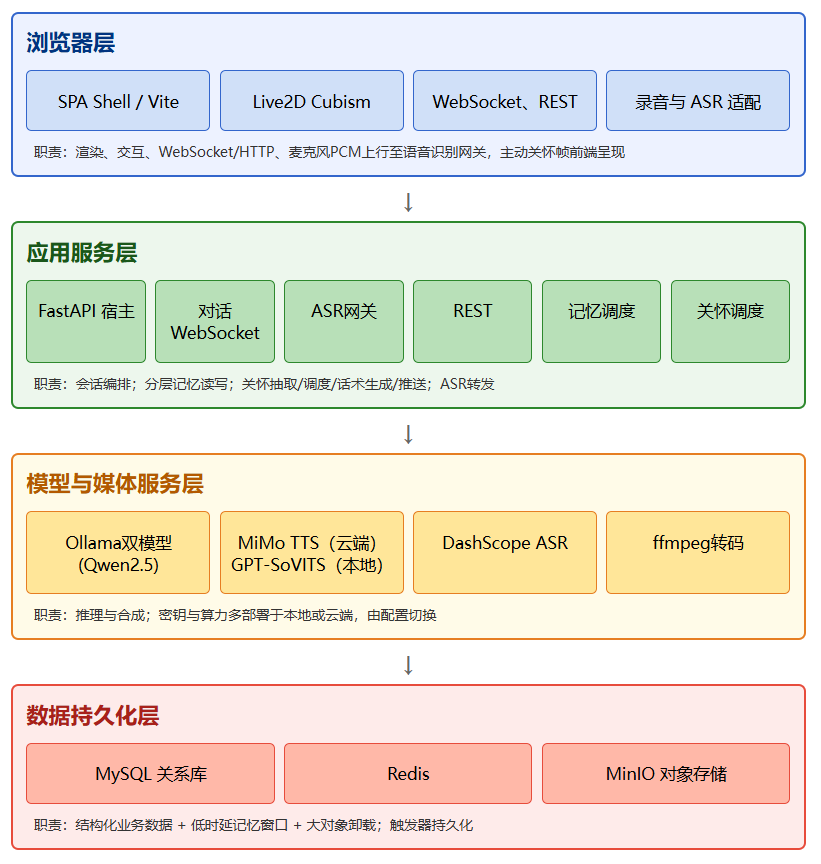
\includegraphics[width=\textwidth]{fig_layer_arch.png}
    \caption{系统四层逻辑架构示意图}
    \label{fig:layer_arch}
\end{figure}

\begin{figure}[htbp]
    \centering
    \resizebox{0.92\textwidth}{!}{
        \begin{tikzpicture}[
                font=\small,
                box/.style={rectangle, draw=black!75, thick, rounded corners=3pt, minimum width=3.1cm, minimum height=1.05cm, align=center},
                arr/.style={-{Latex[length=2.8mm]}, thick},
            ]
            \node[box, fill=blue!6] (fe) at (0,0) {浏览器前端\\[-2pt]{\scriptsize Vite + Cubism}};
            \node[box, fill=green!8] (fa) at (5.4,0) {FastAPI 编排\\[-2pt]{\scriptsize WebSocket / REST}};
            \node[box, fill=orange!10] (ollama) at (10.8,1.35) {Ollama\\[-2pt]{\scriptsize 双模型推理}};
            \node[box, fill=purple!10] (tts) at (10.8,-1.35) {TTS\\[-2pt]{\scriptsize MiMo / 本地}};
            \node[box, fill=gray!12] (data) at (5.4,-3.1) {Redis / MySQL / MinIO\\[-2pt]{\scriptsize 记忆与资源}};
            \node[box, fill=yellow!12] (sch) at (0,-3.1) {关怀调度器\\[-2pt]{\scriptsize 定时扫描}};
            \draw[arr] (fe) -- node[above,font=\scriptsize]{/ws/chat,/ws/asr} (fa);
            \draw[arr] (fa) -- node[above,sloped,font=\scriptsize]{聊天/动作} (ollama);
            \draw[arr] (fa) -- node[below,sloped,font=\scriptsize]{切段合成} (tts);
            \draw[arr] (fa) -- node[right,font=\scriptsize]{读写} (data);
            \draw[arr] (sch) -- node[above,font=\scriptsize]{到期推送} (fa);
        \end{tikzpicture}
    }
    \caption{主要软件模块依赖关系示意}
    \label{fig:module_deps}
\end{figure}

图~\ref{fig:seq_main_dialogue}给出主对话端到端时序。

\begin{figure}[H]
    \centering
    \resizebox{\SeqDiagramWidth}{!}{
        \begin{tikzpicture}[
                font=\footnotesize,
                participant/.style={rectangle, draw=black!70, thick, minimum width=2.35cm, minimum height=0.72cm, align=center, fill=white},
                lifeline/.style={dashed, thick, gray!50},
                msg/.style={-{Latex[length=2.4mm]}, thick},
                retmsg/.style={-{Latex[length=2.4mm]}, thick, dashed},
                note/.style={rectangle, draw=black!35, fill=yellow!10, rounded corners=2pt, font=\footnotesize, inner sep=3pt, align=left},
            ]
            \node[participant] (U)   at (0,   0) {用户};
            \node[participant] (BR)  at (3.2, 0) {浏览器\\[-2pt]{\scriptsize ws.js}};
            \node[participant] (ASR) at (6.2, 0) {ASR网关\\[-2pt]{\scriptsize /ws/asr}};
            \node[participant] (DS)  at (9.0, 0) {DashScope\\[-2pt]{\scriptsize Fun-ASR}};
            \node[participant] (WS)  at (12.0,0) {对话编排\\[-2pt]{\scriptsize /ws/chat}};
            \node[participant] (OL)  at (15.3,0) {Ollama\\[-2pt]{\scriptsize 双模型}};
            \node[participant] (TTS) at (18.2,0) {TTS服务\\[-2pt]{\scriptsize MiMo}};
            \node[participant] (DB)  at (21.0,0) {Redis/MySQL};

            \begin{scope}[yscale=\SeqYScale, transform shape]
            \pgfmathsetmacro{\r}{\SeqRow}
            \foreach \x in {0,3.2,6.2,9.0,12.0,15.3,18.2,21.0}
            \draw[lifeline] (\x,-0.38) -- (\x,-22.0);

            \node[note] at (1.6,-0.95) {\textit{路径A：语音}};
            \pgfmathsetmacro{\yA}{-1.35}
            \draw[msg] (0,\yA) -- node[above,font=\footnotesize]{语音输入} (6.2,\yA);
            \pgfmathsetmacro{\yA}{\yA-\r}
            \draw[msg] (6.2,\yA) -- node[above,font=\footnotesize]{PCM二进制帧} (9.0,\yA);
            \pgfmathsetmacro{\yA}{\yA-\r}
            \draw[retmsg] (9.0,\yA) -- node[above,font=\footnotesize]{识别中间/终稿事件} (6.2,\yA);
            \pgfmathsetmacro{\yA}{\yA-\r}
            \draw[retmsg] (6.2,\yA) -- node[above,font=\footnotesize]{终稿文本回填} (3.2,\yA);

            \pgfmathsetmacro{\yB}{\yA-0.85*\r}
            \node[note] at (1.6,\yB) {\textit{路径B：文本}};
            \pgfmathsetmacro{\yB}{\yB-0.85*\r}
            \draw[msg] (0,\yB) -- node[above,font=\footnotesize]{文本输入} (3.2,\yB);

            \pgfmathsetmacro{\y}{\yB-\r}
            \draw[msg] (3.2,\y) -- node[above,font=\footnotesize]{\texttt{/ws/chat}连接} (12.0,\y);
            \pgfmathsetmacro{\y}{\y-\r}
            \draw[msg] (12.0,\y) -- node[above,font=\footnotesize]{加载catalog+TTS配置} (21.0,\y);
            \pgfmathsetmacro{\y}{\y-\r}
            \draw[retmsg] (21.0,\y) -- node[above,font=\footnotesize]{catalog数据} (12.0,\y);
            \pgfmathsetmacro{\y}{\y-\r}
            \draw[retmsg] (12.0,\y) -- node[above,font=\footnotesize]{\texttt{type:catalog}} (3.2,\y);

            \pgfmathsetmacro{\y}{\y-\r}
            \draw[msg] (3.2,\y) -- node[above,font=\footnotesize]{\texttt{\{"message":"...","scene\_location":"..."\}}} (12.0,\y);

            \pgfmathsetmacro{\y}{\y-\r}
            \draw[msg] (12.0,\y) -- node[above,font=\footnotesize]{读分层记忆+人设+用户画像} (21.0,\y);
            \pgfmathsetmacro{\y}{\y-\r}
            \draw[retmsg] (21.0,\y) -- node[above,font=\footnotesize]{瞬时List/短期List/长期String} (12.0,\y);

            \pgfmathsetmacro{\y}{\y-\r}
            \draw[msg] (12.0,\y) -- node[above,font=\footnotesize]{动作决策} (15.3,\y);
            \pgfmathsetmacro{\y}{\y-\r}
            \draw[retmsg] (15.3,\y) -- node[above,font=\footnotesize]{\texttt{expression/motion} JSON} (12.0,\y);

            \pgfmathsetmacro{\y}{\y-\r}
            \draw[msg] (12.0,\y) -- node[above,font=\footnotesize]{聊天补全 stream=True} (15.3,\y);
            \pgfmathsetmacro{\y}{\y-\r}
            \draw[retmsg] (15.3,\y) -- node[above,font=\footnotesize]{token增量流} (12.0,\y);

            \pgfmathsetmacro{\y}{\y-\r}
            \draw[retmsg] (12.0,\y) -- node[above,font=\footnotesize]{\texttt{chunk}} (3.2,\y);
            \node[note,anchor=west] at (3.35,{\y-0.38*\r}) {\footnotesize setExpression/startMotion控制Live2D};

            \pgfmathsetmacro{\y}{\y-1.05*\r}
            \node[note,anchor=east] at (18.1,{\y-0.35*\r}) {\footnotesize 按句末标点攒批并行worker合成};
            \draw[msg] (12.0,\y) -- node[above,font=\footnotesize]{TTS请求} (18.2,\y);
            \pgfmathsetmacro{\y}{\y-\r}
            \draw[retmsg] (18.2,\y) -- node[above,font=\footnotesize]{WAV音频} (12.0,\y);

            \pgfmathsetmacro{\y}{\y-\r}
            \draw[retmsg] (12.0,\y) -- node[above,font=\footnotesize]{\texttt{chunk\_audio}\{index,size,content\}} (3.2,\y);
            \pgfmathsetmacro{\y}{\y-\r}
            \draw[retmsg,ultra thick] (12.0,\y) -- node[above,font=\footnotesize]{二进制WAV帧} (3.2,\y);
            \node[note,anchor=west] at (3.35,{\y-0.38*\r}) {\footnotesize enqueueAudioAndPlay；RMS$\rightarrow$口型同步};

            \pgfmathsetmacro{\y}{\y-1.1*\r}
            \draw[retmsg] (12.0,\y) -- node[above,font=\footnotesize]{\texttt{type:done}} (3.2,\y);

            \pgfmathsetmacro{\y}{\y-\r}
            \draw[msg] (12.0,\y) -- node[above,font=\footnotesize]{LPUSH瞬时/短期List；写chat\_session} (21.0,\y);
            \node[note,anchor=west] at (12.15,{\y-0.42*\r}) {\footnotesize 每轮异步调用remind\_extract抽取关怀触发器（不阻塞主链路）};
            \node[note,anchor=west] at (12.15,{\y-0.88*\r}) {\footnotesize user\_profile由lifespan后台按24h策略独立刷新（见\S\ref{sec:user_profile}）};

            \pgfmathsetmacro{\yEnd}{\y-1.15*\r}
            \foreach \x in {0,3.2,6.2,9.0,12.0,15.3,18.2,21.0}
            \fill (\x,\yEnd) circle (2.5pt);
            \end{scope}
        \end{tikzpicture}
    }
    \caption{主对话端到端时序图}
    \label{fig:seq_main_dialogue}
\end{figure}

\subsection{主对话端到端时序说明}

图中自上而下共八个纵向参与者：用户侧的输入意图首先落在浏览器脚本层（\texttt{ws.js}）；若走语音识别，则经本域\texttt{/ws/asr}网关转发至云端 DashScope Fun-ASR，再以中间结果与终稿事件回流浏览器完成文本回填；若用户直接键入文本，则跳过 ASR 泳道。两条路径在下文统称为``路径A（语音）''与``路径B（文本）''，汇合后均由浏览器通过已有\texttt{/ws/chat} WebSocket 与会话编排交互，从而保证语音仅改变上游采集形态，不改变下游对话语义通道。

连接稳定后，编排端按需访问 Redis/MySQL：加载当前模型包及 TTS 相关配置，并以\texttt{type:catalog}等形式下发浏览器，使前端具备合法\texttt{expression}/\texttt{motion}索引集合，供后续动作字段校验与回退。用户上行负载为包含\texttt{message}与场景字段等的 JSON；编排据此读取分层记忆（瞬时 List、短期 List、长期字符串），与人设、用户画像、角色锚点及身份区分规则一并拼入单条\texttt{system}（【三种记忆】位于\texttt{system}末段），本轮问题写入单独\texttt{user}，再进入推理阶段。

推理分为两步且顺序固定：先请求动作决策模型得到结构化\texttt{expression}/\texttt{motion}；再对主对话模型发起\texttt{stream=True}的补全调用，将持续返回的 token 增量映射为下行\texttt{chunk}帧。浏览器收到\texttt{chunk}后并行更新字幕，并按帧内字段调用\texttt{setExpression}/\texttt{startMotion}控制 Live2D，实现``台词流式可见、表情动作与文本同源触发''。

朗读链路与文本流交错推进：编排侧按句末标点将待合成文本切段，以并行 worker 请求 TTS（图中 MiMo），但下行仍携带段落序号，保证\texttt{chunk\_audio}元数据与随后的二进制 WAV 帧严格按播放顺序抵达前端；前端将音频入队播放，并可结合 RMS 等信号同步口型，避免``音频先到、台词未到''或段落乱序。

当编排发送\texttt{type:done}标志本轮生成结束时，持久化写回启动：向 Redis 推送瞬时与短期记忆列表项，并向 MySQL 的会话日志（如\texttt{chat\_session}）落库，形成可追溯的对话记录。图中注释标明会话收尾阶段的异步旁路：\texttt{remind\_extract}在每轮持久化后以异步任务抽取关怀触发器，不阻塞用户感知的主链路。用户画像合并则由\texttt{main.py}~lifespan注册的\texttt{user\_profile\_consolidator}独立轮询维护，与本轮\texttt{done}解耦（见第~\ref{sec:user_profile}节）。

% ====================================================
% 第三章 核心模块设计与实现
% ====================================================
\chapter{核心模块设计与实现}

本章按浏览器呈现层、WebSocket协议层、FastAPI编排层、持久化与REST层自顶向下展开，所有文件路径与环境变量默认值均以\path{Demo/}、\path{PY/}代码为准。本章所述能力均面向已登录会话，不提供访客入口。

\section{前端页面、Live2D 与交互实现}

\subsection{布局与登录态}

前端基于Vite组织模块化源码，\texttt{index.html}为单页入口。主界面采用左会话、右角色双栏：左侧集中历史气泡\texttt{\#chat-list}、流式字幕区、文本输入与语音按钮；右侧为WebGL画布与可展开工具条（含模型/背景切换、资源上传、``更新长期记忆''与``更新用户画像''等维护按钮，分别调用对应\texttt{consolidate-now}接口）。已登录用户在三步内完成``输入→等待流式反馈→同步听取朗读''。入口脚本在\texttt{DOMContentLoaded}后校验\texttt{localStorage}中的\texttt{live2d\_info}，缺失则重定向至\texttt{Login.html}。

\subsection{Live2D 组件层级}

\begin{sloppypar}
    图~\ref{fig:live2d_components}以UML组件图风格展示前端Live2D运行时四级层次：\texttt{LAppDelegate}\allowbreak →\texttt{LAppSubdelegate}\allowbreak →\texttt{LAppLive2DManager}\allowbreak →\texttt{LAppModel}。\texttt{ws.js}经\texttt{apply\-Chat\-Live\-2d\-Actions}委托入口控制表情与动作。
\end{sloppypar}

\begin{figure}[htbp]
    \centering
    \resizebox{0.88\textwidth}{!}{
        \begin{tikzpicture}[
                font=\small,
                comp/.style={rectangle, draw=black!70, thick, rounded corners=3pt, minimum width=4.0cm, minimum height=0.7cm, align=center, inner sep=5pt},
                agg/.style={{Diamond[open,length=3mm]}-{Latex[length=2.5mm]}, thick},
                dep/.style={-{Latex[length=2.5mm]}, thick, dashed},
                use/.style={-{Latex[length=2.5mm]}, thick, blue!70},
            ]
            \node[comp, fill=blue!10, minimum width=7.5cm] (delegate) at (5.0, 0)
            {\texttt{LAppDelegate}\\[-2pt]
                \scriptsize 初始化Cubism SDK；管理子代理集合；\\[-2pt]
                \scriptsize 注册全局指针/resize事件；帧循环广播；\texttt{applyChatLive2dActions}委托入口};
            \node[comp, fill=green!8, minimum width=6.5cm] (subdelegate) at (5.0, -3.0)
            {\texttt{LAppSubdelegate}\\[-2pt]
                \scriptsize 持有\texttt{<canvas>}+WebGL上下文；纹理管理；\\[-2pt]
                \scriptsize 画布尺寸/ResizeObserver；指针命中与拖拽};
            \node[comp, fill=orange!8, minimum width=6.0cm] (manager) at (5.0, -6.0)
            {\texttt{LAppLive2DManager}\\[-2pt]
                \scriptsize 维护\texttt{\_models[]}向量；切换ModelDir场景；\\[-2pt]
                \scriptsize 转发drag/tap/\texttt{applyChatLive2dActions}};
            \node[comp, fill=yellow!8, minimum width=5.5cm] (model) at (5.0, -9.0)
            {\texttt{LAppModel}\\[-2pt]
                \scriptsize 加载\texttt{.model3.json}、表情、物理、动作；\\[-2pt]
                \scriptsize \texttt{setExpression(id)}；\texttt{startMotionByBasename}};
            \node[comp, fill=gray!8, minimum width=3.0cm] (define) at (-2.6, -9.0)
            {\texttt{lappdefine.js}\\[-2pt]\scriptsize ModelDir/资源根路径/常量};
            \node[comp, fill=purple!8, minimum width=4.5cm] (wsjs) at (14.5, -4.5)
            {\texttt{ws.js / main.js}\\[-2pt]
                \scriptsize 接收chunk/chunk\_audio；\\[-2pt]
                \scriptsize 解析expression/motion；\\[-2pt]
                \scriptsize Web Audio RMS→口型同步};

            \draw[agg] (subdelegate.north) -- node[right,font=\scriptsize]{1..*} (delegate.south);
            \draw[agg] (manager.north) -- node[right,font=\scriptsize]{1} (subdelegate.south);
            \draw[agg] (model.north) -- node[right,font=\scriptsize]{1..*} (manager.south);
            \draw[dep,shorten <=1mm,shorten >=1mm] (define.east) -- node[midway,above,font=\scriptsize]{使用} (model.west);
            \draw[use,shorten <=1mm,shorten >=1mm] (wsjs.west) -- node[midway,above,sloped,font=\scriptsize,inner sep=1.5pt]{\texttt{applyChatLive2dActions}} (delegate.east);
            \draw[use,dashed] (wsjs.south) -- ++(0,-0.5) -- node[right,font=\scriptsize]{setExpr/startMotion} (model.east);
        \end{tikzpicture}
    }
    \caption{前端Live2D组件层级UML图}
    \label{fig:live2d_components}
\end{figure}

\subsection{远程资源与预签名加载}

\begin{sloppypar}
    私有MinIO桶场景下，已登录用户在\texttt{live2d\_info}校验通过后，由\texttt{main.js}执行：通过\path{GET /api/live2d-model-assets}拉取当前包资产行，对含\texttt{object\_key}的行调用\texttt{download-url}换取限时URL，最后将\texttt{relative\_path→可fetch URL}写入远程manifest供\texttt{LAppModel}拉取。并发解析默认并行上限24，以平衡TLS握手与总等待。
\end{sloppypar}

\subsection{语音输入与对话入口合一}

\begin{sloppypar}
    语音链路单独维护至\path{/ws/asr}。浏览器以\texttt{MediaDevices.\allowbreak{}getUserMedia()}采集麦克风，PCM一般为16\,kHz/16\,bit/单声道，经二进制WebSocket帧上行；服务端\path{PY/router/asr_ws.py}与DashScope Fun-ASR建立实时会话并将事件回写。浏览器在收到终稿后填入输入框并调用与键盘相同的\texttt{sendChatMessage}，从而共用同一对话状态机。
\end{sloppypar}

\section{WebSocket 连接与流式协议}

\subsection{地址推导与查询参数语义}

\begin{sloppypar}
    \texttt{wsConfig.js}优先读取\texttt{VITE\_WS\_BASE}；否则由\texttt{VITE\_API\_BASE}推导\texttt{ws}/\texttt{wss}与主机端口；二者皆空时回退\texttt{ws://localhost:8000}。对话URL由\texttt{getChatWsUrl()}拼接\texttt{session}、\texttt{package}与\texttt{user\_id}三类查询参数：\texttt{session}为标签页级会话键，存\texttt{sessionStorage}并与MySQL \texttt{chat\_session.session\_key}对齐；\texttt{package}与\path{Demo/public/Resources/<package>}目录名一致；\texttt{user\_id}与已登录账户一致，供后端加载绑定的音色参考与人设等。
\end{sloppypar}

\subsection{下行帧类型与朗读捆绑格式}

\begin{sloppypar}
    表~\ref{tab:ws_chat_frames}归纳\path{/ws/chat}上主要JSON类型字段时间顺序。二进制帧规则：仅当紧前一条JSON为\texttt{chunk\_audio}时，下一条二进制才被视作WAV；否则丢弃并告警。\texttt{ws.binaryType="arraybuffer"}，解码后进入Web Audio调度链，按\texttt{index}从小到大依次播放。
\end{sloppypar}

\begin{table}[htbp]
    \centering
    \caption{\texttt{/ws/chat}主要JSON类型与前端处理要点}
    \label{tab:ws_chat_frames}
    \begingroup
    \small
    \sloppy
    \setlength{\tabcolsep}{8pt}
    \renewcommand{\arraystretch}{1.36}
    \begin{tabularx}{\textwidth}{@{} >{\raggedright\arraybackslash}p{2.85cm} Y Y @{}}
        \toprule
        \textbf{type}         & \textbf{载荷要点}                                             & \textbf{浏览器侧行为}                                                  \\
        \midrule
        \path{catalog}        & 包键；可用表情、动作名及路径列表                                          & 控制台诊断；供开发与\path{catalog}对照                                       \\
        \path{chunk}          & 文本增量字段\path{content}；首包可附带\path{expression}与\path{motion} & 流式拼接字幕与气泡文本；解析表情与动作并控制Live2D                                     \\
        \path{chunk_audio}    & \path{index}、\path{size}；对应朗读文本段；部分场景首段可带头套动作字段           & 缓存本条音频元数据；随后一条消息须为二进制帧，按\path{index}从小到大依次入队播放                   \\
        \path{remind_trigger} & 含\path{trigger_content}、\path{delivery_message}等          & 气泡展示采用\path{delivery_message}；若开启关怀朗读可继续收到\path{chunk_audio}与二进制 \\
        \path{done}           & 标记本轮对话结束                                                  & 合并气泡；清理本轮等待状态                                                    \\
        \path{error}          & 含可读\path{message}                                         & 界面提示错误；解除发送锁定                                                    \\
        \bottomrule
    \end{tabularx}
    \endgroup
\end{table}

\subsection{断线重连、模型切换与消息打断}

\begin{sloppypar}
    客户端在\texttt{onclose}中以常量\texttt{RECONNECT\_MS=3000}定义的固定间隔调度重连。切换模型时主动\texttt{close}并递增\texttt{skipAutoReconnectCount}，避免\texttt{onclose}触发的自动重连与手动换包重连叠加。\texttt{onmessage}首行比对\texttt{event.target===textSocket}，丢弃旧socket上迟到的JSON/二进制，防止换包或打断后字幕、音频错位入队。重连后\id{flush_pending_reminders_for_connection}会将该用户离线期间到期的关怀触发器补发。
\end{sloppypar}

\section{服务端对话编排}

\subsection{应用生命周期}

\path{PY/main.py}使用FastAPI \texttt{lifespan}：启动阶段调用\texttt{init\_catalog()}预热表情动作索引；\texttt{await}~\id{start_long_memory_consolidator()}挂载长期记忆后台循环；\texttt{await}~\id{start_user_profile_consolidator()}挂载用户画像24小时合并后台任务；\texttt{await}~\id{start_remind_trigger_scheduler()}启动关怀触发器常驻扫描任务。关闭阶段对称停止上述任务。CORS默认放行常见Vite开发端口，并允许通过环境变量\texttt{CORS\_ORIGINS}追加生产前端源。

\subsection{一轮对话内的编排流水线}

\begin{sloppypar}
    每收到非空\texttt{message}，编排顺序概括为：1.~记忆与人设拼装，按\path{PY/live2d_db/memory_layers.py}约定读取Redis列表与字符串、必要时回填MySQL长期概要，拼接system/user消息；2.~动作决策，在线程池中对\texttt{OLLAMA\_ACTION\_MODEL}做一次非流式补全，解析\texttt{expression}/\texttt{motion}，经集合校验与回退后附着于首段文本chunk；3.~聊天生成，对聊天模型启用\texttt{stream=True}，通过\texttt{asyncio.Queue}与事件循环线程桥接；4.~朗读，按句末标点攒批，分段并行请求TTS，合并流模式下以\texttt{chunk\_audio}+WAV按序号依次下发；5.~收尾，发送\texttt{done}，持久化本轮对话至MySQL，更新Redis瞬时/短期列表，在\texttt{REMIND\_EXTRACT\_FROM\_DIALOGUE}开启且用户已登录时每轮异步触发\texttt{remind\_extract}关怀抽取（\texttt{remind\_extract\_turn\_should\_run}对合法\texttt{user\_id}恒为真，已不再按\texttt{N}轮节流）。用户画像刷新不在本步同步触发，而由\texttt{user\_profile\_consolidator}后台任务按24小时策略维护（见第~\ref{sec:user_profile}节）。
\end{sloppypar}

\begin{sloppypar}
    上述第4步在实现上可概括为图~\ref{fig:tts_pipeline}：聊天token缓冲至句末标点或上限后入\texttt{sentence\_queue}，由\texttt{tts\_worker}经\texttt{asyncio.to\_thread}并行合成，结果写入\texttt{tts\_completed}后由\id{_tts_flush_ordered}按序号经WebSocket下发\texttt{chunk\_audio}与二进制WAV，对应\path{PY/router/wschat.py}中三段协作。
\end{sloppypar}

\begin{figure}[htbp]
    \centering
    \resizebox{0.9\textwidth}{!}{
        \begin{tikzpicture}[
                font=\small,
                box/.style={rectangle, draw=black!70, thick, rounded corners=3pt, minimum width=3.2cm, minimum height=0.75cm, align=center, inner sep=5pt},
                diam/.style={diamond, draw=black!70, thick, aspect=2.5, minimum width=3.8cm, minimum height=0.8cm, align=center, inner sep=2pt},
                arr/.style={-{Latex[length=2.5mm]}, thick},
                darr/.style={-{Latex[length=2mm]}, thick, dashed},
            ]
            \node[box, fill=blue!8] (tok) at (0,0) {Ollama token\\[-2pt]写入缓冲区};
            \node[diam, fill=orange!10, below=0.5cm of tok] (chk) {句末标点计数\\[-2pt]$\geq N$或token上限？};
            \node[box, fill=gray!8, right=1.2cm of chk] (cont) {继续缓冲};
            \node[box, fill=green!10, below=0.8cm of chk] (enq) {index自增\\[-2pt]文本段入sentence\_queue};
            \node[box, fill=blue!8, below=0.7cm of enq] (worker) {tts\_worker取\\[-2pt]index与text};
            \node[box, fill=blue!8, below=0.5cm of worker] (synth) {asyncio.to\_thread\\[-2pt]调用TTS合成};
            \node[box, fill=green!10, below=0.5cm of synth] (store) {tts\_completed[index]\\[-2pt]$\leftarrow$ text与WAV};
            \node[box, fill=orange!8, below=0.6cm of store] (flush) {调用\_tts\_flush\_ordered()};
            \node[diam, fill=orange!10, below=0.5cm of flush] (rdy) {tts\_next\_send\\[-2pt]已就绪？};
            \node[box, fill=gray!8, right=1.2cm of rdy] (wait) {等待更小\\[-2pt]序号就绪};
            \node[box, fill=green!10, below=0.8cm of rdy] (send) {send\_json(chunk\_audio)\\[-2pt]+ send\_bytes(WAV)};
            \node[box, fill=blue!8, below=0.5cm of send] (inc) {tts\_next\_send += 1};

            \draw[arr] (tok) -- (chk);
            \draw[arr] (chk) -- node[left,font=\scriptsize]{是} (enq);
            \draw[darr] (chk) -- node[above,font=\scriptsize]{否} (cont);
            \draw[darr] (cont.south) |- ++(0,-0.3) -| (tok.east);
            \draw[arr] (enq) -- (worker);
            \draw[arr] (worker) -- (synth);
            \draw[arr] (synth) -- (store);
            \draw[arr] (store) -- (flush);
            \draw[arr] (flush) -- (rdy);
            \draw[arr] (rdy) -- node[left,font=\scriptsize]{是} (send);
            \draw[darr] (rdy) -- node[above,font=\scriptsize]{否} (wait);
            \draw[arr] (send) -- (inc);
            \draw[darr] (inc.east) -- ++(0.5,0) |- (flush.east);
        \end{tikzpicture}
    }
    \caption{TTS切段、并行合成与按序号依次下发流程}
    \label{fig:tts_pipeline}
\end{figure}

\section{数据持久化、REST API 与资源管理}

\subsection{MySQL 核心表结构}

\begin{sloppypar}
    业务库当前共九张表，均由\path{PY/live2d_db/schema.sql}定义：其中八张与用户或会话主数据存在外键关联，依次为\texttt{user}（鉴权）、\texttt{persona}（人设）、\texttt{live2d\_model\_asset}（模型文件元数据与对象存储键）、\texttt{live2d\_tts\_refer}（按用户+模型包唯一的参考音频绑定，供 GPT-SoVITS 等路径读取\texttt{prompt\_text}/\texttt{prompt\_language}及音频定位信息）、\texttt{user\_profile}（画像）、\texttt{chat\_session}（对话轮次）、\texttt{long\_memory}（长期概要）及\texttt{remind\_trigger}（主动关怀触发器）；第九张\texttt{background\_image}仅存场景背景图的逻辑名与对外可访问URL，实体文件在MinIO桶内，表侧无外键，用作全局背景资源索引；前端通过\path{GET /api/background-images/random}等接口取\path{name}/\path{url}换肤。历史增量脚本\path{PY/live2d_db/migrations/20260508_background_image.sql}与schema中该表段落一致，可供仅有旧库时单独补表。图~\ref{fig:db_er}用简化实体框列出全部九张表及外键箭头（由子表指向父表主键）；\texttt{background\_image}与其他表之间无连线表示无外键。列级定义见表~\ref{tab:background_image_fields}、表~\ref{tab:live2d_tts_refer_fields}；\texttt{remind\_trigger}各字段见后文表~\ref{tab:remind_trigger_fields}。上述两张单列表明细与彼表列示体例一致。
\end{sloppypar}

\begin{sloppypar}
    各表角色简述如下。\texttt{user}保存账号凭证与基础资料，是下列多张表的外键锚点。\texttt{persona}存放人设正文及语气字段，可选绑定到\texttt{user\_id}+模型包键，用于对话\texttt{system}拼装。\texttt{live2d\_model\_asset}按用户与包键索引Live2D切片文件及对象存储键，支撑\texttt{catalog}校验与预签名加载。\texttt{live2d\_tts\_refer}绑定用户与包键级的参考音频元数据，供合成路径选用。\texttt{user\_profile}每用户一行画像字段（含\texttt{display\_name}称呼），由24小时后台合并任务与可选即时接口维护。\texttt{chat\_session}持久化单轮用户输入与助手回复及会话键，是审计与长期概要生成的数据源。\texttt{long\_memory}按用户与包键聚合周期概要正文。\texttt{remind\_trigger}存放到期时间与抽取情景，\texttt{session\_id}可空并外键指向\texttt{chat\_session}，便于投递话术时回溯产生该触发的对话语境；用户删除采用\texttt{ON DELETE CASCADE}级联清理依附行，会话删除对触发器采用\texttt{ON DELETE SET NULL}以免破坏历史审计语义。\texttt{background\_image}仅存背景显示名与对外URL，与其他表无强制外键。
\end{sloppypar}

% ✅ 已替换为 SVG 格式 ER 总图（保持原尺寸、标签、引用不变）
\begin{figure}[htbp]
    \centering
    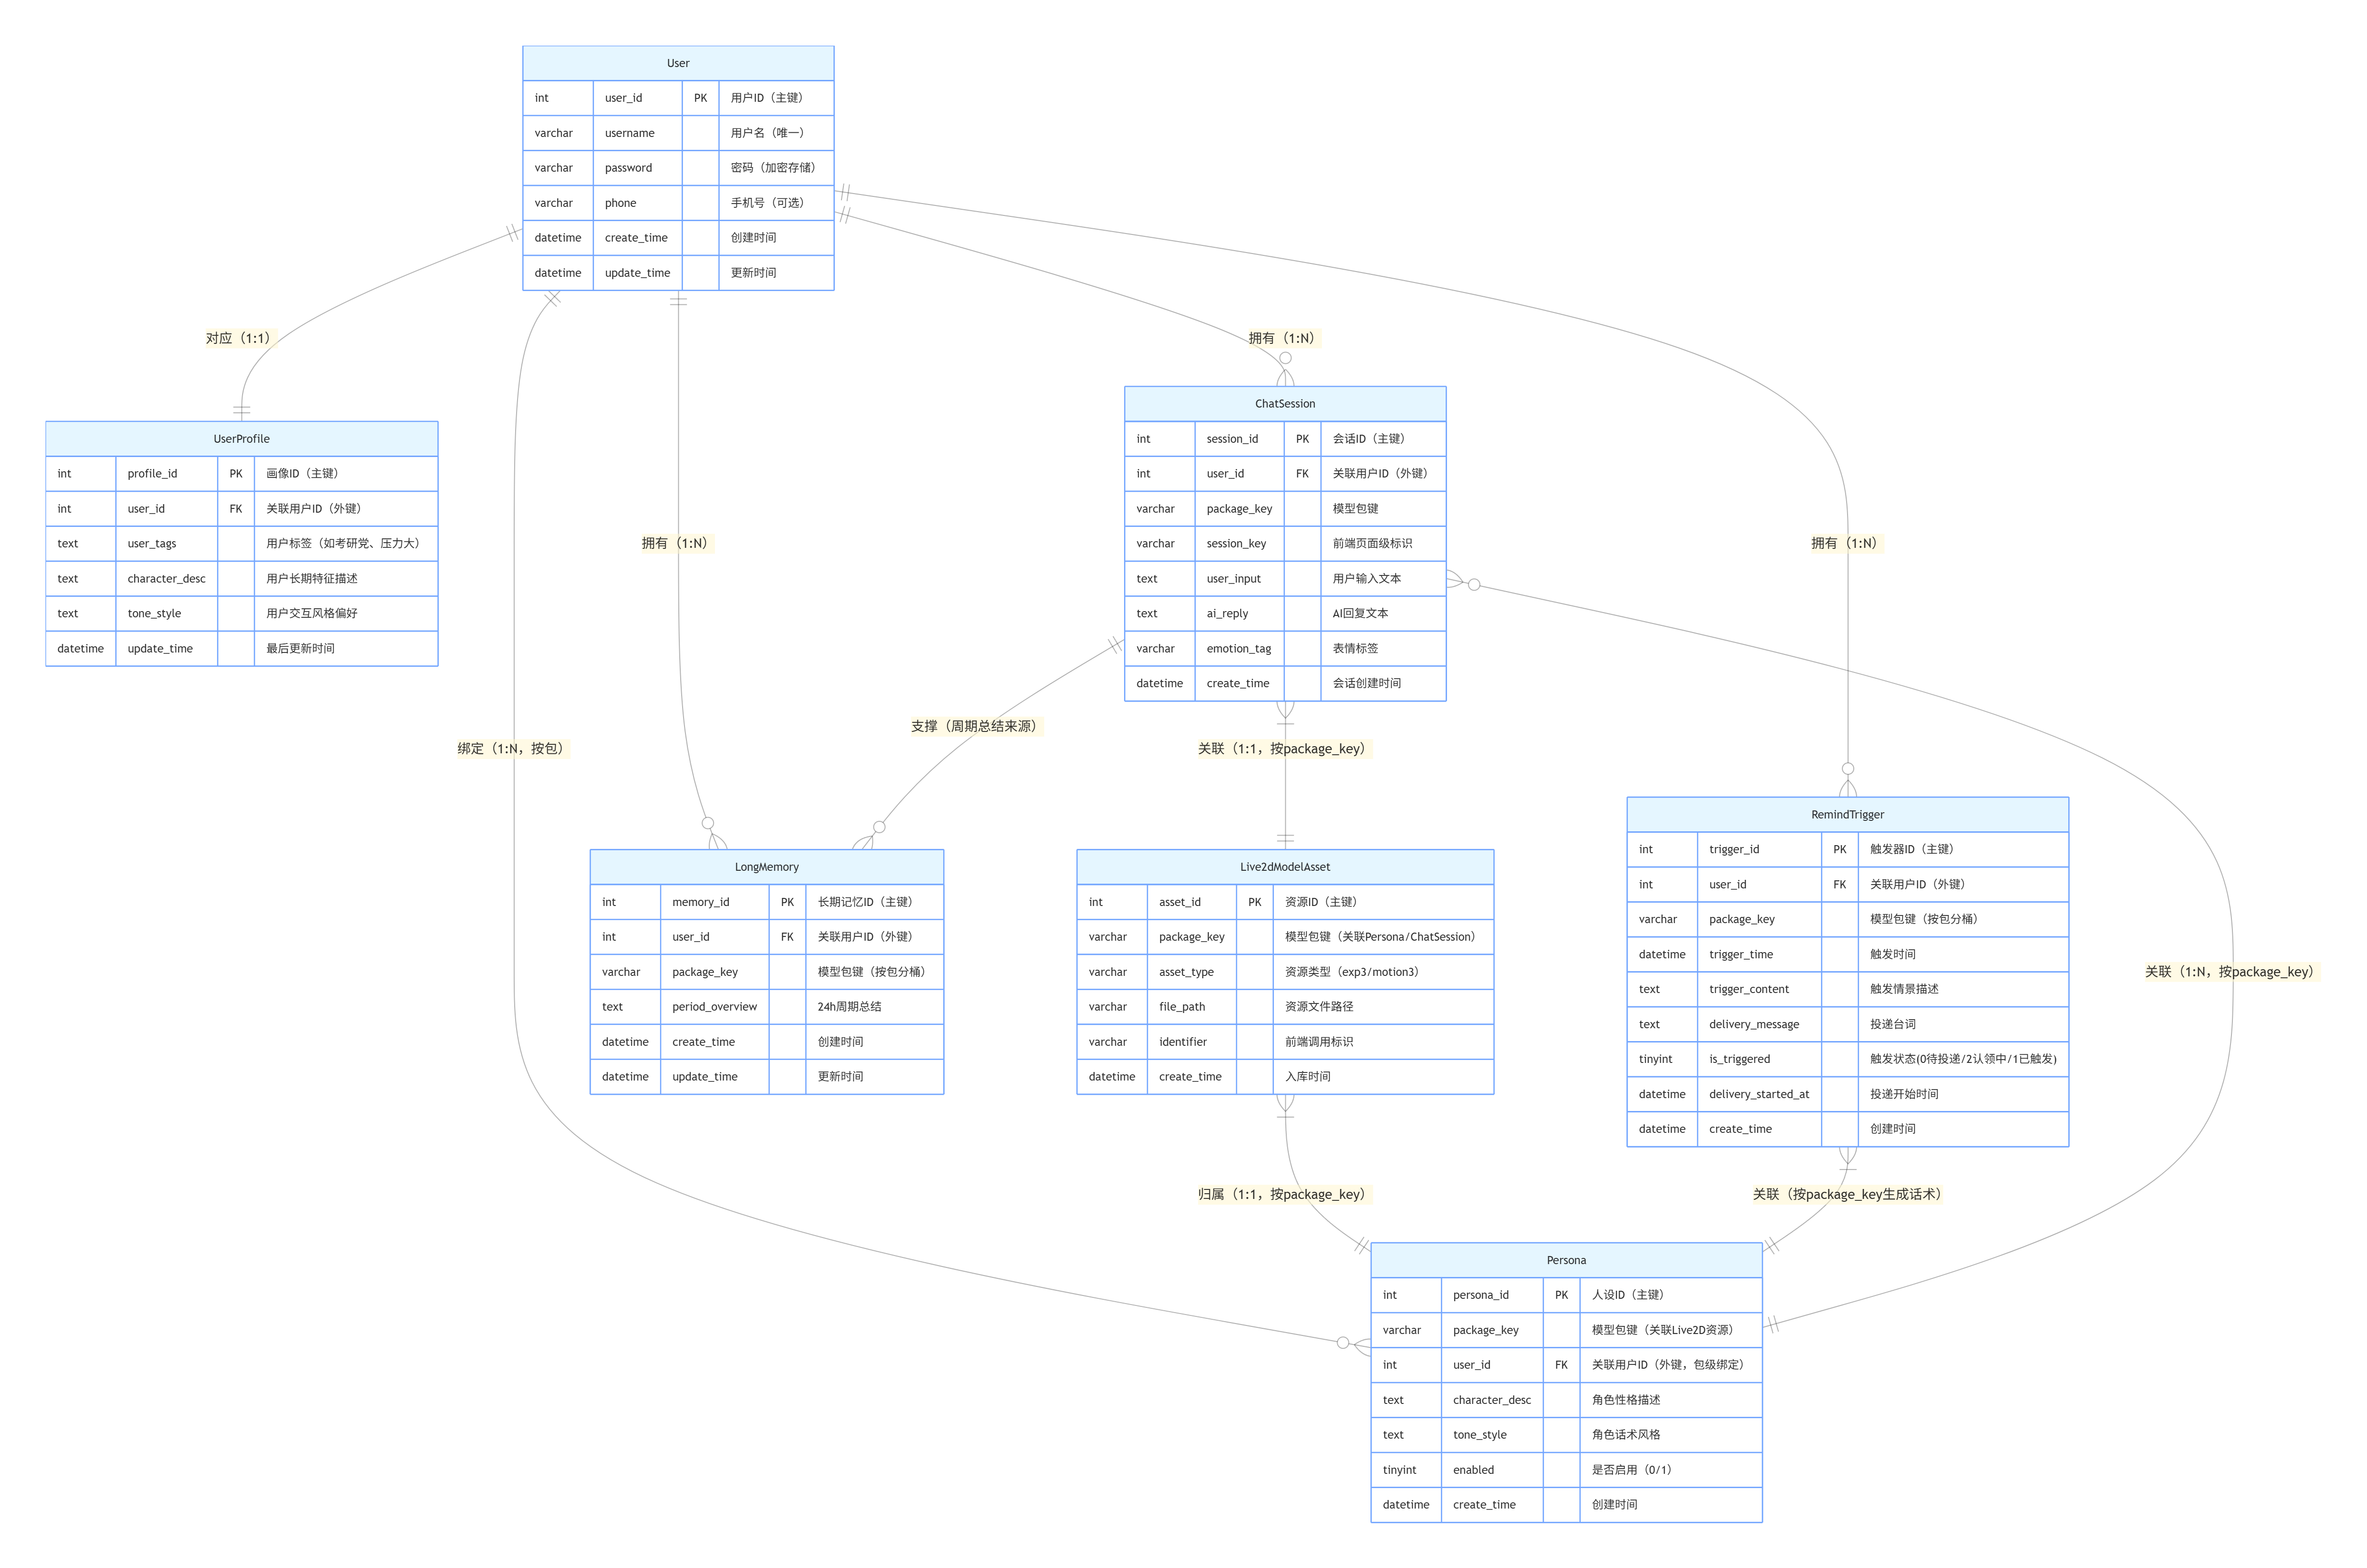
\includegraphics[width=\textwidth]{fig_er_diagram.png}
    \caption{MySQL九张主链路核心表简化ER关系图}
    \label{fig:db_er}
\end{figure}

\begin{table}[htbp]
    \centering
    \caption{\texttt{background\_image}表字段说明}
    \label{tab:background_image_fields}
    \begingroup
    \small
    \sloppy
    \setlength{\tabcolsep}{7pt}
    \renewcommand{\arraystretch}{1.36}
    \begin{tabularx}{\textwidth}{@{} >{\raggedright\arraybackslash}p{2.85cm} >{\raggedright\arraybackslash}p{2.75cm} Y @{}}
        \toprule
        \textbf{字段名}      & \textbf{类型/约束} & \textbf{含义}                                      \\
        \midrule
        \path{id}         & BIGINT PK        & 主键                                                 \\
        \path{name}       & VARCHAR(512) UK  & 显示名/逻辑名，不含扩展名                                     \\
        \path{url}        & VARCHAR(1024)    & MinIO 对外访问 URL，供前端换肤与随机背景接口返回                    \\
        \path{create_time}& DATETIME         & 索引行写入时间                                           \\
        \bottomrule
    \end{tabularx}
    \endgroup
\end{table}

\begin{table}[htbp]
    \centering
    \caption{\texttt{live2d\_tts\_refer}表字段说明}
    \label{tab:live2d_tts_refer_fields}
    \begingroup
    \small
    \sloppy
    \setlength{\tabcolsep}{7pt}
    \renewcommand{\arraystretch}{1.36}
    \begin{tabularx}{\textwidth}{@{} >{\raggedright\arraybackslash}p{3.25cm} >{\raggedright\arraybackslash}p{2.75cm} Y @{}}
        \toprule
        \textbf{字段名}               & \textbf{类型/约束}           & \textbf{含义}                                                          \\
        \midrule
        \path{refer_id}            & BIGINT PK                & 参考音频绑定行 ID                                                         \\
        \path{user_id}             & INT FK→user, UK 组合键之一   & 所属用户                                                               \\
        \path{package_key}         & VARCHAR(64), UK 组合键之一   & 模型包键；与 \path{user_id} 联合唯一，每用户每包一条                                   \\
        \path{audio_object_key}    & VARCHAR(768) NULL          & MinIO 对象键                                                           \\
        \path{audio_url}           & VARCHAR(1024) NULL         & 参考音频 URL（可为预签名临时链接）                                                \\
        \path{audio_format}        & VARCHAR(16) NULL           & 音频格式，如 wav/mp3                                                     \\
        \path{prompt_text}         & VARCHAR(512)               & GPT-SoVITS 参考文本 \path{prompt_text}                                  \\
        \path{prompt_language}     & VARCHAR(32)                & GPT-SoVITS 参考语种 \path{prompt_language}                              \\
        \path{create_time}         & DATETIME                   & 创建时间                                                               \\
        \path{update_time}         & DATETIME                   & 更新时间                                                               \\
        \bottomrule
    \end{tabularx}
    \endgroup
\end{table}

\subsection{REST 路由分组与统一响应封装}
\path{PY/live2d_db/http_api.py}共注册59条\texttt{/api}路由。自定义\texttt{UnifiedResponseRoute}在路由处理层封装响应：成功时统一\texttt{code=0}、\texttt{message=ok}、\texttt{data}为业务载荷；失败时\texttt{code}取HTTP状态码、\texttt{message}为错误描述、\texttt{data=null}，便于前端单一解析逻辑。接口按业务模块划分为8个功能分组，具体实现如下：

\subsubsection*{用户与画像分组}
REST接口在\texttt{users}与\texttt{user-profiles}分组内提供完整用户及画像管理能力，例如：
\begin{itemize}\setlength{\itemsep}{2pt}\setlength{\parsep}{0pt}
    \item \path{POST /api/users}：完成用户注册与登录，支持用户名、密码校验及信息创建；
    \item \path{GET /api/users/resolve}：通过手机号或邮箱唯一解析用户公开信息；
    \item \path{GET /api/user-profiles/by-user/{user_id}}：查询指定用户的完整画像数据；
    \item \path{POST /api/user-profiles/consolidate-now}：立即合并用户画像（近24小时内全部\texttt{chat\_session}，跨模型包），跳过后台24小时最短间隔。
\end{itemize}

\subsubsection*{会话与长期记忆分组}
REST接口在\texttt{chat-sessions}、\texttt{long-memories}分组内实现对话记录与记忆管理，例如：
\begin{itemize}\setlength{\itemsep}{2pt}\setlength{\parsep}{0pt}
    \item \path{POST /api/chat-sessions}：写入单轮对话会话记录，包含用户输入与AI回复；
    \item \path{POST /api/long-memories/consolidate-now}：立即触发长期记忆滚动合并（增量摘要与库内概要合并或压缩堆叠），跳过后台24小时最短间隔。
\end{itemize}

\subsubsection*{角色人设分组}
REST接口在\texttt{personas}分组内提供Live2D角色人设配置能力，例如：
\begin{itemize}\setlength{\itemsep}{2pt}\setlength{\parsep}{0pt}
    \item \path{GET /api/personas/by-package/{package_key}}：按模型包查询绑定的角色人设；
    \item \path{POST /api/personas/expand-from-hints}：根据提示词自动扩写生成角色人设内容。
\end{itemize}

\subsubsection*{模型资产分组}
REST接口在\texttt{live2d-model-assets}分组内实现模型文件的上传与下载，例如：
\begin{itemize}\setlength{\itemsep}{2pt}\setlength{\parsep}{0pt}
    \item \path{POST /api/live2d-model-assets/upload-zip}：通过ZIP包批量上传Live2D模型资源；
    \item \path{GET /api/live2d-model-assets/download-url}：生成模型资产的预签名下载链接。
\end{itemize}

\subsubsection*{语音配置分组}
REST接口在\texttt{live2d-tts-refers}分组内提供语音合成配置管理，支持TTS参数与音色的增删改查。

\subsubsection*{定时关怀分组}
REST接口在\texttt{remind-triggers}分组内提供完整CRUD及若干诊断入口，例如：
\begin{itemize}\setlength{\itemsep}{2pt}\setlength{\parsep}{0pt}
    \item \path{GET /api/remind-triggers/pending-scan}：拉取截至当前时刻仍未触发且已到期的记录列表；
    \item \path{GET /api/remind-triggers/pending-count}：返回与上一接口筛选条件一致的条数；
    \item \path{POST /api/remind-triggers/scan-now}：不等后台周期，立即执行一轮扫描；响应体\path{data}中带\path{pending_fetched}、\path{delivered}、\path{released_no_ws}等计数，便于区分``无到期行''与``用户不在线未下发''等情形。
\end{itemize}

\subsubsection*{背景资源分组}
REST接口在\texttt{background-images}分组内管理界面背景资源，例如：
\begin{itemize}\setlength{\itemsep}{2pt}\setlength{\parsep}{0pt}
    \item \path{GET /api/background-images/random}：随机返回一张可用的背景图片名称与访问链接。
\end{itemize}

\begin{table}[htbp]
    \centering
    \caption{REST关键接口示例}
    \label{tab:rest_key_examples}
    \begingroup
    \footnotesize
    \sloppy
    \setlength{\tabcolsep}{6pt}
    \renewcommand{\arraystretch}{1.34}
    \begin{tabularx}{\textwidth}{@{} >{\raggedright\arraybackslash}p{3.35cm} >{\raggedright\arraybackslash}p{2.25cm} Y Y @{}}
        \toprule
        \textbf{Method/Path}                             & \textbf{语义} & \textbf{请求要点}                                                                                & \textbf{\texttt{data}载荷要点}                                                                           \\
        \midrule
        \path{POST /api/users}                           & 注册用户        & JSON：\path{username}、\path{password}；可选\path{nickname}等                                      & 新建用户的\path{user_id}与公开字段                                                                             \\
        \path{GET /api/users/resolve}                    & 按手机号或邮箱解析   & Query：\path{phone=}与\path{email=}二选一                                                         & 用户公开信息                                                                                               \\
        \path{POST /api/chat-sessions}                   & 写入会话轮次      & JSON：\path{user_id}、\path{package_key}、\path{user_input}、\path{ai_reply}、\path{session_key}等 & 会话行\path{session_id}及时间戳                                                                             \\
        \path{GET /api/live2d-model-assets/download-url} & 资产预签名URL    & Query：\path{asset_id}、可选\path{expires_in}                                                    & \path{url}、过期相关字段                                                                                    \\
        \path{POST /api/live2d-model-assets/upload-zip}  & ZIP批量入库     & Form：\path{user_id}；可选\path{package_key}；File：\path{model_zip}，扩展名为.zip                      & 包键、导入条目数与跳过文件统计等摘要字段                                                                                 \\
        \path{POST /api/long-memories/consolidate-now}   & 触发长期滚动合并    & Query：\path{user_id}必填；可选\path{package_key}                                                  & \path{ok}、\path{updated}（无增量且无需压缩时可为假）                                                  \\
        \path{POST /api/user-profiles/consolidate-now}   & 立即合并用户画像    & Query：\path{user_id}必填                                                                        & \path{ok}、\path{updated}（24h窗内无对话或LLM结果为空时可为假）                                         \\
        \path{POST /api/remind-triggers/scan-now}        & 立即扫描到期关怀    & 无请求体                                                                                         & \path{pending_fetched}、\path{claimed}、\path{delivered}、\path{released_no_ws}、\path{stale_reclaimed}等 \\
        \path{GET /api/background-images/random}         & 随机背景        & 一般无参数                                                                                        & 单条背景\path{name}、\path{url}                                                                           \\
        \bottomrule
    \end{tabularx}
    \endgroup
\end{table}

\subsection{ZIP 入库与删除一致性}

\path{POST /api/live2d-model-assets/upload-zip}解压校验、推断包名、批量写MinIO与\texttt{live2d\_model\_asset}；删除包时移除对象与索引行，并清理依附\texttt{persona}及Redis缓存，保证再次连接\path{/ws/chat}时catalog与存储一致。

% ====================================================
% 第四章 分层记忆系统设计与实现
% ====================================================
\chapter{分层记忆系统设计与实现}

\section{理论参照}

\subsection{阿特金森--谢弗林多层存储模型}

认知心理学中的阿特金森--谢弗林多层存储模型由Atkinson与Shiffrin系统阐述\cite{Atkinson1968}：记忆不是单一扁平仓库，而是在时间上串联的多级结构。外界信息先进入极短暂的感觉登记，经注意进入容量有限的短时存储，继而在复述、编码等控制过程作用下转入保持更久的长时存储，以供日后检索与利用。

本文立场：上文关于三级结构的概括用于读者定位本文瞬时/短期/长期三联设计的叙述来源，绝不等于在计算机里复制感官生理过程或复述短时容量等心理学定量结论。表~\ref{tab:memory_analogy}给出工程对应与类比边界说明。

\begin{table}[htbp]
    \centering
    \caption{阿特金森--谢弗林三级结构与本文三层记忆的叙述类比}
    \label{tab:memory_analogy}
    \begingroup
    \small
    \setlength{\tabcolsep}{8pt}
    \renewcommand{\arraystretch}{1.4}
    \begin{tabularx}{\textwidth}{@{} Y Y Y @{}}
        \toprule
        \textbf{心理学层级}         & \textbf{本文工程对应}                              & \textbf{类比边界说明}                 \\
        \midrule
        感觉登记：极短保持的感觉缓冲         & 人机采集层PCM、ASR流式中间结果等                          & 仅作入口缓冲的类比说明；无感官生理学仿真          \\
        短时存储：容量/时间受限，复述有助于转入长时 & 瞬时List最近$K$轮与短期List挤出后的规则条目                  & 容量由常量与TTL约束；``复述''对应规则压缩，而非心理复述 \\
        长时存储：相对持久、可提取          & \texttt{long\_memory}周期概要于MySQL与Redis长期字符串缓存 & 非完整语义记忆理论实现；强调可注入、可审计、可失效TTL    \\
        \bottomrule
    \end{tabularx}
    \endgroup
\end{table}

\subsection{MemGPT 的工程类比}

MemGPT的基本思路是：大模型单次能读进去的字数有限，不可能把全部历史原封不动塞进每次请求；因此把当下真正拼进prompt的一小段与篇幅更长、存放在外部的记录分开——后者落在数据库或向量库等外部存储里，对话进行中再按需读取、拼接或摘要写回，从而在不要求单次prompt无限变长的前提下延续多轮一致性\cite{MemGPT2023}。

与MemGPT相比，本文面对同一问题：上下文长度有限，却又要利用更早的对话与人设。因此在存储上同样分为``当轮注入块''与``外部存放块''：前者主要是最近若干轮原文及短期压缩条目，后者落在Redis列表、字符串或MySQL字段，由编排代码在固定步骤读取或更新。

本文未采用MemGPT中由模型自主决定读写时机的做法，原因在于本科教学场景更需可复现、可对照日志的确定性路径，故何时写Redis、何时读MySQL概要均固定在编排代码的常见路径里。其余差异包括：其一，调度层不用操作系统式复杂换页，而以可配置的Redis List与TTL完成裁剪；其二，长期层以MySQL字段中的文本概要为主，而非向量检索，以便数据留在本库、便于审计。

\section{三层架构设计}\label{sec:memgptrelation}

图~\ref{fig:memory_arch}展示三层记忆的存储介质、数据形态与注入方式。

\begin{figure}[htbp]
    \centering
    \resizebox{0.95\textwidth}{!}{
        \begin{tikzpicture}[
                font=\small,
                layer/.style={rectangle, draw=black!70, thick, rounded corners=4pt, minimum width=13cm, inner sep=10pt},
                sublabel/.style={font=\bfseries\small, anchor=north west},
                detail/.style={font=\scriptsize, anchor=north west},
                arr/.style={-{Latex[length=3mm]}, thick},
            ]
            \node[layer, fill=blue!8] (instant) at (0,0) {
                \begin{minipage}{12.6cm}
                    \textbf{瞬时记忆层}\\[2pt]
                    \scriptsize 存储介质：Redis List，键前缀默认\texttt{moment}，空闲TTL默认3600\,s\\
                    \scriptsize 数据形态：JSON元素\texttt{\{"u":"用户发言","a":"助手回复","ts":"时间戳"\}}，每元素一轮\\
                    \scriptsize 容量策略：\texttt{LPUSH}新轮入头，\texttt{LTRIM}保留最近$K$轮，默认$K=5$\\
                    \scriptsize 注入方式：格式化为纯文本，写入主对话\texttt{system}内【三种记忆】的「最近对话」段（\texttt{system}末段紧贴本轮\texttt{user}）\\
                    \scriptsize 动作LLM：独立读取同一瞬时List，注入专用标签模型\texttt{user}侧（不含短期/长期全文）
                \end{minipage}
            };
            \node[layer, fill=green!8, below=0.4cm of instant] (short) {
                \begin{minipage}{12.6cm}
                    \textbf{短期记忆层}\\[2pt]
                    \scriptsize 存储介质：Redis List，键前缀默认\texttt{short}，单键TTL默认86400\,s\\
                    \scriptsize 数据形态：两类条目——规则压缩条\texttt{type:rule}与摘要条\texttt{type:summary}，结构预留\\
                    \scriptsize 容量策略：最多20条，常量\id{SHORT_TERM_MAX_ENTRIES}；拼入system的字符上限默认4000\\
                    \scriptsize 写入时机：瞬时List溢出时，被\texttt{LTRIM}挤出的最旧轮经\id{rule_compact_turn}规则压缩后\texttt{LPUSH}入本层\\
                    \scriptsize 注入方式：\texttt{LRANGE}后从新到旧格式化为纯文本，写入【三种记忆】的「近期摘要」段
                \end{minipage}
            };
            \node[layer, fill=orange!8, below=0.4cm of short] (longm) {
                \begin{minipage}{12.6cm}
                    \textbf{长期记忆层}\\[2pt]
                    \scriptsize 存储介质：MySQL \texttt{long\_memory.period\_overview}类型TEXT与Redis String缓存，键前缀\texttt{long}，TTL默认604800\,s\\
                    \scriptsize 数据形态：\texttt{period\_overview}为单段滚动概要（近期对话脉络）；本窗增量摘要经LLM与旧文合并替换，禁止分隔符堆叠\\
                    \scriptsize 更新时机：后台\path{long\_memory\_consolidator.py}按\texttt{last\_consolidate\_time}增量读\texttt{chat\_session}（24\,h滑动窗）；轮询默认300\,s，同用户×包最短间隔24\,h；\path{consolidate-now}可即时触发或压缩历史堆叠\\
                    \scriptsize 注入方式：读Redis String，未命中回填MySQL；拼入上限默认2000字符，超长保留文尾；称呼/偏好等见用户画像，长期段不重复
                \end{minipage}
            };

            \draw[arr] (instant.south) -- node[right,font=\scriptsize]{溢出轮次经规则压缩} (short.north);
            \draw[arr] (short.south) -- node[right,font=\scriptsize]{周期概要后台任务} (longm.north);
        \end{tikzpicture}
    }
    \caption{三层记忆架构：均折叠入主对话单条system的【三种记忆】块；短期经规则压缩；长期由后台任务滚动合并并缓存于Redis}
    \label{fig:memory_arch}
\end{figure}

\section{瞬时记忆：Redis List 读写机制}

\subsection{JSON 元素格式与 LPUSH/LTRIM 策略}

每轮对话结束后，\id{_append_turn_memory_layers}执行下列写入：

\begin{verbatim}
算法 瞬时记忆写入
输入: user_id, package_key, 本轮用户文本 U, 助手文本 A
1. 构造 JSON 轮次 R ← {"u":U, "a":A, "ts":now()}
2. LPUSH instant_key(user, pkg), R
3. LTRIM instant_key 保留最近 K 轮         // 默认 K=5
4. 若本轮挤出最旧轮 E:
5.     E' ← rule_compact_turn(E)          // 截断+敷衍过滤
6.     LPUSH short_key, E'
7.     对 short_key 执行条数裁剪与 TTL 续期
输出: 更新后的 Redis 状态
\end{verbatim}

\subsection{注入主对话上下文的方式}

主对话每轮仅向 Ollama 提交一条\texttt{system}与一条\texttt{user}。\id{_build_memory_for_model}通过\id{read_instant_turns_chronological}读取瞬时List，与短期、长期文本一并经\id{_format_three_memories_block}写入\texttt{system}末段【三种记忆】（块内顺序为瞬时、短期、长期，并声明冲突优先级）；人设、场景、用户画像及\id{_chat_role_anchor}、\id{_chat_identity_rules}等置于\texttt{system}前部。本轮用户输入在\id{ollama_chat_messages}中格式化为\texttt{【当前用户问题】}并附加回复长度约束。超长时\id{_build_and_trim_main_chat_system}按短期、长期、瞬时轮数递减裁剪。这使模型在单条\texttt{system}内仍能``看见''最近$K$轮完整原文，且与长期脉络共处一段可控上下文。

\subsection{动作 LLM 对瞬时记忆的独立使用}

动作/表情选型模型为单独一次非流式调用，与主对话并行发起；其\texttt{system}为资源表与人设任务说明，\texttt{user}侧由\id{_live2d_tag_llm_user_content_sync}拼装瞬时记忆、场景与本轮用户输入。不注入短期或长期记忆，亦不注入用户画像块。选型语义明确：\texttt{expression}/\texttt{motion}表示Live2D虚拟角色（助手）应切换到的资源，不是真人用户的表情或动作。

\section{短期记忆：规则压缩与 system 拼装}

\subsection{规则压缩算法}

被\texttt{LTRIM}挤出的最旧轮次经\id{rule_compact_turn}处理：对用户句与助手句分别做长度截断；若助手回复为敷衍应答，极短且无实质内容，则清空\texttt{ai\_response}字段。压缩后条目形态为：

\begin{verbatim}
{
  "type": "rule",
  "time": "2026-05-08T10:30:00+00:00",
  "user_question": "截断后的用户句",
  "ai_response": "截断后的助手句，敷衍时为空"
}
\end{verbatim}

\subsection{摘要条目结构预留}

短期List亦可存放\texttt{type:summary}条目：默认由\path{PY/utils/short_term_summary.maybe_push_short_term_summary_after_turn}在\path{/ws/chat}每轮写Redis后按独立计数键每\texttt{N}轮（默认5，可配置）调用Ollama生成摘要并调用\id{push_summary_entry}，环境变量控制，默认关闭；亦可由业务侧直接调用\id{push_summary_entry}。结构形态为\texttt{\{"type":"summary","time":...,"text":"摘要正文"\}}。写入时可从短期List中移除\texttt{type==rule}且时间落在\id{prune_rule_turn_times}内的条目，避免摘要与规则条重复占用上下文。\path{SHORT_TERM_SUMMARY_ENABLED=1}开启内置周期摘要，默认为关闭以免额外占用推理。

\subsection{system 拼装与字符上限控制}

\id{_build_memory_for_model}生成的\texttt{system}由\id{_assemble_main_chat_system_content}拼装：角色锚点与身份区分规则→【角色人设】\texttt{tone\_style}/\texttt{character\_desc}→【角色场景】/【用户时间】→【用户画像】（含\texttt{display\_name}称呼，注明描述真人用户；维护时禁止将角色名写入\texttt{display\_name}或\texttt{user\_tags}）→【三种记忆】（瞬时/短期/长期三段及冲突说明）。长期段默认2000字符且保留文尾，短期段默认4000；预算超限时\id{_build\_and\_trim\_main\_chat\_system}优先裁短期、再长期、最后减少瞬时轮数。历史不再展开为多条\texttt{user/assistant}；本轮问题单独占一条\texttt{user}。

\section{长期记忆：周期概要后台任务}

\subsection{long\_memory\_consolidator 调度机制}

后台任务\path{PY/live2d_db/long_memory_consolidator.py}由\path{PY/main.py}的\texttt{lifespan}调用\id{start_long_memory_consolidator}挂载：默认每300秒轮询候选（\texttt{LONG\_MEMORY\_SCAN\_POLL\_INTERVAL\_SEC}），由\id{list_candidates_for_consolidation}对同一用户×包施加最短24小时合并间隔，执行\id{consolidate_one}：

\begin{enumerate}
    \item 以\texttt{last\_consolidate\_time}为\texttt{since\_exclusive}，在24小时滑动窗内增量读取\texttt{chat\_session}（\id{list_for_long_memory_window}）；无新行且无需压缩堆叠概要时跳过；
    \item 增量会话改写为口述式叙述，Ollama生成本窗摘要（约5--8句，侧重进行中话题；稳定事实不写重复，见用户画像）；
    \item 与库内已有\texttt{period\_overview}经第二轮LLM滚动合并为单段（约6--10句）替换写入；若检测到历史分隔符堆叠或超长，可先仅压缩旧文；
    \item \id{upsert_by_user_pkg}写MySQL，\id{write_long_memory_text}刷新Redis；库内字段上限默认5000字符（\texttt{LONG\_MEMORY\_DB\_MAX\_CHARS}）。
\end{enumerate}

\subsection{即时周期概要更新接口}

\begin{sloppypar}
    \path{POST /api/long-memories/consolidate-now}对指定\texttt{user\_id+package\_key}调用同一套\id{consolidate_one}，在\texttt{asyncio.to\_thread}中执行以免阻塞事件循环；不受后台24小时最短间隔限制，便于开发期手动触发或前端工具栏``更新长期记忆''（滚动合并/压缩堆叠）调用。用户画像的即时合并接口见第~\ref{sec:user_profile}节。
\end{sloppypar}

\section{用户画像：user\_profile 的生成与注入}
\label{sec:user_profile}

\subsection{触发条件与 LLM 合并机制}

\begin{sloppypar}
    用户画像\texttt{user\_profile}每\texttt{user\_id}一行，字段包含\texttt{display\_name}（用户自称/常用称呼）、\texttt{user\_tags}、\texttt{emotion\_state}、\texttt{preferences}、\texttt{trouble\_events}。称呼仅写入\texttt{display\_name}，\texttt{user\_tags}不重复称呼；近期话题流水账由长期记忆\texttt{period\_overview}维护，画像侧不写重复。刷新由\path{PY/utils/user_profile_refresh.py}中\texttt{user\_profile\_consolidator}后台任务负责（\path{main.py}~lifespan启动，默认每300秒扫描）：近24小时内\texttt{chat\_session}有对话且距上次\texttt{update\_time}已满24小时时，以旧画像与自上次更新以来、落在24小时窗内的跨\texttt{package\_key}增量会话为材料调用LLM合并后\texttt{upsert}至MySQL；连续多日无对话不触发，不在回归首日补跑历史堆叠。
\end{sloppypar}

\begin{sloppypar}
    \path{POST /api/user-profiles/consolidate-now}对指定\texttt{user\_id}调用同一套\id{consolidate_user_profile}（\texttt{manual=True}），在\texttt{asyncio.to\_thread}中执行；取材近24小时内全部会话且跨模型包，不受后台24小时最短间隔限制，便于开发期手动触发或前端工具栏``更新用户画像''按钮调用。响应\texttt{data.updated}表示是否成功写入画像（窗内无对话或LLM结果为空时为假）。
\end{sloppypar}

\subsection{画像与人设的分列设计原则}

用户画像记录真人用户的标签与偏好，人设约束虚拟角色的性格与语气；二者主语不同，若写入同一段，模型易把用户事实当成角色自述，或把角色口吻写成对用户档案的复述。因此在\id{_assemble_main_chat_system_content}中将二者分成【用户画像】与【角色人设】两段，并在提示中注明身份区分规则。

人设字段描述的是跨场次稳定的角色设定；而每轮对话还有随包的场景信息（如用户上行 JSON 中的\texttt{scene\_location}）。若把可变场景也塞进人设段，会迫使频繁改库且易与人设混淆。故除人设外，另从\texttt{background\_image}表随机取背景名写入【角色场景】块，仅提供轻量氛围，不覆盖\texttt{scene\_location}所表达的具体地点。

上述分列同样用于关怀话术生成：\texttt{remind\_delivery}分别读取人设与用户画像，避免到期推送时角色口吻漂移。用户画像是否注入可由环境变量\texttt{USER\_PROFILE\_IN\_CHAT}关闭，默认开启；未来若扩展世界观等长文本，仍可沿用``人设一块、画像一块、场景一块''的拼装顺序，无需改动记忆读写主路径。

\section{分层记忆整体读写流程}

图~\ref{fig:memory_flow}展示服务端在一轮对话中读取并组装记忆上下文于轮首以及轮末将本轮对话写回各层存储的完整流程。

\begin{figure}[htbp]
    \centering
    \resizebox{0.95\textwidth}{!}{
        \begin{tikzpicture}[
                font=\small,
                box/.style={rectangle, draw=black!70, thick, rounded corners=3pt, minimum width=3.5cm, minimum height=0.7cm, align=center, inner sep=4pt},
                redbox/.style={rectangle, draw=red!60, thick, rounded corners=3pt, fill=red!5, minimum width=3.5cm, minimum height=0.7cm, align=center, inner sep=4pt},
                sqlbox/.style={rectangle, draw=blue!60, thick, rounded corners=3pt, fill=blue!5, minimum width=3.5cm, minimum height=0.7cm, align=center, inner sep=4pt},
                arr/.style={-{Latex[length=2.5mm]}, thick},
                darr/.style={-{Latex[length=2mm]}, thick, dashed, gray!70},
            ]
            \node[box, fill=blue!8] (start) at (0,0) {收到用户消息};
            \node[redbox] (inst) at (-4.5,-2) {读瞬时List\\[-2pt]\texttt{moment:*}最近K轮};
            \node[redbox] (short) at (0,-2) {读短期List\\[-2pt]\texttt{short:*}最多20条};
            \node[redbox] (longr) at (4.5,-2) {读长期String\\[-2pt]\texttt{long:*}以往对话概要};
            \node[sqlbox] (longm) at (4.5,-3.5) {Redis未命中\\[-2pt]回填MySQL \texttt{long\_memory}};
            \node[box, fill=green!8] (assem) at (0,-5.0) {拼装system/user\\[-2pt]记忆上下文};
            \node[box, fill=orange!8, below=0.6cm of assem] (infer) {调用Ollama\\[-2pt]动作决策+对话生成};
            \node[box, fill=blue!8, below=0.6cm of infer] (done) {对话轮结束\\[-2pt]\texttt{type:done}};
            \node[redbox] (winst) at (-4.5,-10.5) {LPUSH瞬时List\\[-2pt]LTRIM保留K轮};
            \node[redbox] (wshort) at (0,-10.5) {被挤出轮次\\[-2pt]规则压缩入短期List};
            \node[sqlbox] (wmysql) at (4.5,-10.5) {持久化\\[-2pt]\texttt{chat\_session}};
            \node[sqlbox] (wlong) at (2.0,-12.2) {后台任务周期\\[-2pt]写\texttt{long\_memory.period\_overview}};
            \node[redbox] (wlongr) at (2.0,-13.5) {刷新Redis\\[-2pt]长期String缓存};

            \draw[arr] (start) -- ++(-4.5,-1.3) -- (inst);
            \draw[arr] (start) -- (short);
            \draw[arr] (start) -- ++(4.5,-1.3) -- (longr);
            \draw[darr] (longr) -- (longm);
            \draw[darr] (longm.south) |- ++(0,-0.3) -| (assem.east);
            \draw[arr] (inst) |- (assem.west);
            \draw[arr] (short) -- (assem);
            \draw[arr] (longr) |- (assem.east);
            \draw[arr] (assem) -- (infer);
            \draw[arr] (infer) -- (done);
            \draw[arr] (done) -- ++(-4.5,-1.3) -- (winst);
            \draw[arr] (done) -- (wshort);
            \draw[arr] (done) -- ++(4.5,-1.3) -- (wmysql);
            \draw[darr] (winst.south) |- ++(0,-0.5) -- (wshort.south);
            \draw[darr] (wmysql.south) |- (wlong);
            \draw[arr] (wlong) -- (wlongr);
        \end{tikzpicture}
    }
    \caption{分层记忆读写流程图}
    \label{fig:memory_flow}
\end{figure}

% ====================================================
% 第五章 主动关怀系统设计与实现
% ====================================================
\chapter{主动关怀系统设计与实现}

\section{设计动机：从被动对话到定时主动关怀}

第四章的分层记忆解决的是``用户再次开口时，角色能否接续前文''；但若用户在对话中提及考试、生日等将来时刻，主对话在当轮应答结束后便不再运行，记忆本身无法在约定时刻主动向用户发消息。为补上这一缺口，本章在\texttt{chat\_session}落库之后增加异步抽取与定时扫描：把将来时刻写入\texttt{remind\_trigger}，到期再由调度器经既有\path{/ws/chat}连接推送，从而把交互从``仅在被询问时响应''扩展为``到期可触达''。

图~\ref{fig:care_loop}据此将上述能力拆为四步：记忆写入、对话内抽取、到期扫描、话术生成与推送。

\begin{figure}[htbp]
    \centering
    \resizebox{0.82\textwidth}{!}{
        \begin{tikzpicture}[
                font=\small,
                stepbox/.style={rectangle, draw=black!70, thick, rounded corners=6pt, minimum width=3.5cm, minimum height=1.4cm, align=center, inner sep=6pt},
                arr/.style={-{Latex[length=3mm]}, ultra thick, gray!60},
            ]
            \node[stepbox, fill=blue!10]  (s1) at (0,  0)    {\textbf{1.记忆存储}\\[-2pt]\scriptsize 对话内容写入\\[-2pt]\scriptsize 瞬时/短期/长期\\[-2pt]\scriptsize 三级记忆与user\_profile};
            \node[stepbox, fill=orange!10](s2) at (6.5,0)    {\textbf{2.信息抽取}\\[-2pt]\scriptsize remind\_extract\\[-2pt]\scriptsize 异步从对话中\\[-2pt]\scriptsize 抽取结构化提醒};
            \node[stepbox, fill=green!10] (s3) at (6.5,-4.5) {\textbf{3.定时扫描}\\[-2pt]\scriptsize 后台调度器\\[-2pt]\scriptsize 周期扫描到期\\[-2pt]\scriptsize 触发器并认领};
            \node[stepbox, fill=purple!10](s4) at (0,-4.5)   {\textbf{4.生成与推送}\\[-2pt]\scriptsize remind\_delivery\\[-2pt]\scriptsize LLM生成话术\\[-2pt]\scriptsize WebSocket投递};

            \draw[arr] (s1.east) -- node[above,font=\scriptsize]{对话落库后异步} (s2.west);
            \draw[arr] (s2.south) -- node[right,font=\scriptsize]{触发器入库} (s3.north);
            \draw[arr] (s3.west) -- node[above,font=\scriptsize]{到期认领} (s4.east);
            \draw[arr] (s4.north) -- node[left,font=\scriptsize,align=right]{用户接收关怀\\记忆更新} (s1.south);
        \end{tikzpicture}
    }
    \caption{主动关怀系统四步流程设计}
    \label{fig:care_loop}
\end{figure}

\section{对话内关怀信息抽取}

每轮对话\texttt{chat\_session}成功落库后，\path{PY/router/wschat.py}异步调用\path{PY/utils/remind_extract.py}，由LLM以本轮用户消息与助手回复为唯一日程事实来源（提示词文首另注入服务器当前时间与\texttt{scene\_time}解析得到的语境参考时间），判断是否写入\texttt{remind\_trigger}并绑定刚插入行的 \texttt{session\_id}。抽取 LLM 另拼装 MySQL 人设绑定与\texttt{persona}正文（仅用于角色指称一致，禁止据此捏造本轮未口述的日程）；不注入 Redis 瞬时记忆与短期记忆，也不读取 MySQL 长期摘要（\texttt{long\_memory.period\_overview}）。

抽取结果写入\texttt{remind\_trigger}的字段语义如下：\texttt{trigger\_type}经服务端规范化后仅当属于生日、纪念日、考试三者之一时才入库；模型若显式输出``其他''等与三类不符的占位\texttt{trigger\_type}，源码计入\texttt{skipped\_explicit\_other}并跳过本条；其余无法识别类型计入\texttt{skipped\_bad\_type}。库内仍可能存在历史上写入的``日常关怀''等遗留行；新抽取路径不再写入日常关怀。\texttt{trigger\_time}为应触发的时刻；\texttt{trigger\_content}存情景概要：须仅以本轮两段正文为事实依据，不得写入仅存在于人设或多轮记忆中的细节；客观叙述须覆盖用户时间、用户地点（未提及时写``地点未提及''等占位）、角色、事件与氛围；供触发当日\texttt{remind\_delivery}生成台词参考（投递侧可另用人设、瞬时记忆等，见第\ref{sec:delivery}节）。\texttt{session\_id}关联产生该提醒的单轮\texttt{chat\_session}。\texttt{is\_triggered}初始为\texttt{0}；调度器认领后为\texttt{2}，WebSocket成功下发含非空\texttt{delivery\_message}的JSON后再置\texttt{1}，详见第~\ref{sec:remind_claim_finish}节。

\section{触发器数据结构与 REST 接口}

\texttt{remind\_trigger}表是主动关怀的核心数据结构，完整字段见表~\ref{tab:remind_trigger_fields}。

\begin{table}[htbp]
    \centering
    \caption{\texttt{remind\_trigger}表字段说明}
    \label{tab:remind_trigger_fields}
    \begingroup
    \small
    \sloppy
    \setlength{\tabcolsep}{7pt}
    \renewcommand{\arraystretch}{1.36}
    \begin{tabularx}{\textwidth}{@{} >{\raggedright\arraybackslash}p{3.25cm} >{\raggedright\arraybackslash}p{2.75cm} Y @{}}
        \toprule
        \textbf{字段名}               & \textbf{类型/约束}                & \textbf{含义}                                                     \\
        \midrule
        \path{trigger_id}          & BIGINT PK                     & 触发器唯一ID                                                         \\
        \path{user_id}             & INT FK→user                   & 关联用户                                                            \\
        \path{session_id}          & BIGINT FK→\path{chat_session} & 产生该提醒的对话轮次，用于话术生成时读取关联上下文                                       \\
        \path{trigger_type}        & VARCHAR(30)                   & 触发类型：新入库主要为生日/纪念日/考试；库内可见历史日常关怀等遗留值                             \\
        \path{trigger_time}        & DATETIME                      & 应触发的时刻，到达此时刻且未成功投递前才纳入扫描                                        \\
        \path{trigger_content}     & TEXT                          & 库内存情景概要（用户时间、地点、角色、事件、氛围五项，未知项占位）；JSON 中与 REST/WebSocket 字段同名同义 \\
        \path{is_triggered}        & TINYINT                       & 投递状态：0 待投递；2 投递中；1 已成功下发或可确认的跳过，与调度实现一致                         \\
        \path{delivery_started_at} & DATETIME NULL                 & 投递中起始时刻，用于超时回收；详见源码                                             \\
        \path{create_time}         & DATETIME                      & 写入时间                                                            \\
        \bottomrule
    \end{tabularx}
    \endgroup
\end{table}

REST接口在\texttt{remind-triggers}分组内提供完整CRUD及若干诊断入口，例如：
\begin{itemize}\setlength{\itemsep}{2pt}\setlength{\parsep}{0pt}
    \item \path{GET /api/remind-triggers/pending-scan}：拉取截至当前时刻仍未触发且已到期的记录列表；
    \item \path{GET /api/remind-triggers/pending-count}：返回与上一接口筛选条件一致的条数；
    \item \path{POST /api/remind-triggers/scan-now}：不等后台周期，立即执行一轮扫描；响应体\path{data}中带\path{pending_fetched}、\path{delivered}、\path{released_no_ws}等计数，便于区分``无到期行''与``用户不在线未下发''等情形。
\end{itemize}

\section{后台调度器}

\subsection{常驻扫描机制}

\path{PY/main.py}的\texttt{lifespan}启动\path{PY/live2d_db/remind_trigger_scheduler.py}，按间隔轮询到期行，默认300秒，可在\path{PY/.env}调小至最小5秒，便于联调；扫描条件与\texttt{GET pending-scan}使用同一套仓储方法\id{list_pending_before}：即\texttt{is\_triggered=0}且\texttt{trigger\_time<=服务器当前时间}。

\subsection{到期与扫描发现的两阶段语义}\label{sec:two_phase}

定时关怀不是在\texttt{trigger\_time}某一时刻由独立闹钟线程精确唤醒，而是同时满足以下两点才对用户可见：

\begin{enumerate}
    \item 到期条件：表中该行\texttt{is\_triggered=0}，且\texttt{trigger\_time<=服务器当前时间}。若面试定在6月15日09:00，在此时间之前无论如何点击扫描，都会出现``当前无到期未触发记录''——这是预期行为。
    \item 发现条件：在满足上列第一点之后，还须经过一次扫描：后台定时任务或\path{POST /api/remind-triggers/scan-now}。因此推送时刻是``到期之后的下一次扫描''，存在至多约一个扫描间隔的滞后，默认约5分钟；联调可缩短扫描间隔，或将测试数据的\texttt{trigger\_time}设为``几分钟前''再点立即扫描。
\end{enumerate}

离线用户：若在无在线\path{/ws/chat}时将行直接标为\texttt{1}，数据库会显示已投递而用户实际未收到。故无连接时不置\texttt{1}；认领后为\texttt{2}，发送失败则\id{release_remind_delivery}回\texttt{0}；用户重连时由\id{flush_pending_reminders_for_connection}按同一投递链路补发，成功后再置\texttt{1}。

\subsection{关怀投递的状态：待投递、处理中与已成功}\label{sec:remind_claim_finish}

若仅凭用户当前是否有在线与满足到期条件就把记录从\texttt{0}直接改为\texttt{1}，容易把连着服务器误当成用户已经收到关怀 JSON：连接尚在时发送仍可能失败；从扫描任务到生成话术、组帧、发送也有时间窗，其间用户可能已断开。另有多轮扫描或并发 worker 时，需要避免同一条到期记录被重复拾取、重复投递。

因此实现上用三步区分。\texttt{0}（待投递）：已到期且未被占用。\texttt{2}（投递中）：调度器调用\id{begin_remind_delivery}，在数据库中将该行一次性从\texttt{0}改为\texttt{2}并写入\texttt{delivery\_started\_at}，表示「本条正由当前流程处理」，在话术生成与发送完成之前不会被别的扫描周期再次当成待投递行。\texttt{1}（已成功）：仅当WebSocket已成功下发含非空\texttt{delivery\_message}的\texttt{remind\_trigger} JSON后，由\id{finish_remind_delivery}置\texttt{1}，表示对用户侧已确认下发成功。

用户不在线、没有可发正文、发送失败等情况，由\id{release_remind_delivery}将\texttt{2}收回\texttt{0}，下次扫描可再试。若进程崩溃或异常中断，记录可能长时间停在\texttt{2}；每轮扫描起始的超时回收逻辑按环境变量\id{REMIND_DELIVERY_STALE_SECONDS}把过久卡在\texttt{2}的行重置为\texttt{0}，避免永久既不能投递又被误认为「正在处理」。

\section{关怀话术生成}\label{sec:delivery}

\subsection{输入拼装}

\path{PY/utils/remind_delivery.py}在调度器成功认领后被调用，其输入拼装顺序为写入LLM的User消息：

\begingroup
\sloppy
\begin{enumerate}
    \item 人设块：MySQL \texttt{persona}，通过\id{_persona_mysql_block}(\id{user_id}, \id{pkg})读取\texttt{tone\_style}/\texttt{character\_desc}；
    \item 用户画像块：当\texttt{USER\_PROFILE\_IN\_CHAT}未关闭且\texttt{user\_profile}存在非空字段时，由\id{format_profile_for_chat_system}格式化为【用户画像】段落，便于生成关怀台词时参考用户背景；
    \item 当前对话瞬时记忆：与同连接\path{/ws/chat}主对话相同分桶键\texttt{user\_id}与\texttt{package\_key}，从Redis瞬时List按时间顺序读取最近多轮\texttt{user}/\texttt{assistant}原文；不拼接短期压缩层条目；
    \item 关怀类型：\texttt{trigger\_type}；
    \item 情景概要：库内\texttt{trigger\_content}（时间、地点、角色、事件、氛围五项备忘）；无则写``未提供''；
    \item 关联对话原文：通过\texttt{session\_id}读取\texttt{chat\_session}的\texttt{user\_input}/\texttt{ai\_reply}；无有效\texttt{session\_id}时写``未绑定''。
\end{enumerate}
\endgroup

\begin{sloppypar}
    LLM系统提示要求重新撰写对用户当场说出的一段话：第一人称、禁止小说式第三人称叙述角色自身；以情景与瞬时对话为主轴，可呼应关联单轮与人设/画像；输出为1～3句口语化中文、不编造材料中不存在的事实、禁止JSON/Markdown格式；输出长度上限约800字符，超出截断加``…''。
\end{sloppypar}

\begin{sloppypar}
    若环境变量\texttt{REMIND\_DELIVERY\_USE\_LLM}关闭为\texttt{0}/\texttt{false}/\texttt{no}/\texttt{off}之一，或情景文本与关联\texttt{session\_id}对话块及Redis瞬时记忆三者皆空以致无法拼装有意义的模型输入，或Ollama调用异常及剥离后的模型输出为空，则\id{generate_remind_delivery_message}返回空串；\id{_deliver_remind_trigger_on_websocket}据此不下发\texttt{remind\_trigger}帧并按调度语义将\texttt{is\_triggered}退回待投递，语义见第~\ref{sec:remind_claim_finish}节。人设或画像读取失败时当前实现记录日志并仍以已有材料尝试调用模型。
\end{sloppypar}

落库与瞬时记忆：WebSocket 已成功下发含非空\texttt{delivery\_message}的\texttt{remind\_trigger} JSON 后，\path{PY/router/wschat.py} 中 \id{_persist_remind_delivery_to_chat_session} 将当场台词写入 MySQL \texttt{chat\_session}：\texttt{user\_input} 留空，\texttt{ai\_reply} 为 \texttt{delivery\_message}；并调用 \id{_append_turn_memory_layers} 更新 Redis 瞬时列表（不经由画像或短期摘要调度）。用户多条 \path{/ws/chat} 连接时仅在首次成功下发的连接上入库一行，避免重复。

\section{WebSocket 推送与 TTS 朗读}

\subsection{type:remind\_trigger 帧格式}

认领成功后，\id{broadcast_remind_trigger_to_user}向该\texttt{user\_id}当前所有\path{/ws/chat}连接发送：

\begin{verbatim}
{
  "type": "remind_trigger",
  "trigger_id": <int>,
  "trigger_type": "<类型>",
  "trigger_content": "<库内情景概要（含用户时间、地点、角色、事件、氛围）>",
  "delivery_message": "<当场LLM生成的面向用户台词>",
  "trigger_time": "<ISO时间>"
}
\end{verbatim}

\begin{sloppypar}
    前端\texttt{ws.js}收到\texttt{type:remind\_trigger}且\texttt{delivery\_message}非空时，仅调用\texttt{appendChatMessage("ai", delivery\_message)}追加角色侧气泡，与库表\texttt{user\_input}为空、\texttt{ai\_reply}为台词一致；样式同普通\texttt{chat-item.ai}。
\end{sloppypar}

\subsection{可选 MiMo 语音朗读}

\begin{sloppypar}
    若MiMo已在\path{PY/.env}完整配置且未关闭``关怀语音''开关，则在\texttt{type:remind\_trigger}帧之后，再按该连接\texttt{package}的参考音与人设导演下发\texttt{chunk\_audio}，含\texttt{remind\_audio:true}标记，以及二进制WAV，朗读内容与JSON中\texttt{delivery\_message}一致，与合并流聊天同一代码路径。关闭开关则仅保留文字气泡，音频不下发。
\end{sloppypar}

\subsection{离线用户重连补发}

用户离线期间到期的触发器记录保持\texttt{is\_triggered=0}，认领失败后释放。当用户重新建立\path{/ws/chat}连接时，\id{flush_pending_reminders_for_connection}被调用，以\id{list_pending_for_user_before}传入\texttt{now}读取所有属于该用户的到期未触发记录，依次走与常驻扫描相同的认领→话术生成→投递链路，确保用户不会因短暂离线而错过关怀消息。

\section{主动关怀端到端时序}

图~\ref{fig:care_seq}展示从对话落库到WebSocket推送的完整时序，涵盖抽取、调度、话术生成与推送四个阶段。

\begin{figure}[H]
    \centering
    \resizebox{\SeqDiagramWidth}{!}{
        \begin{tikzpicture}[
                font=\footnotesize,
                participant/.style={rectangle, draw=black!70, thick, minimum width=2.55cm, minimum height=0.72cm, align=center, fill=white},
                lifeline/.style={dashed, thick, gray!50},
                msg/.style={-{Latex[length=2.4mm]}, thick},
                retmsg/.style={-{Latex[length=2.4mm]}, thick, dashed},
                note/.style={rectangle, draw=black!35, fill=yellow!10, rounded corners=2pt, font=\footnotesize, inner sep=3pt, align=left},
            ]
            \node[participant] (dial) at (0,0)    {对话编排\\[-2pt]{\scriptsize /ws/chat}};
            \node[participant] (ext)  at (4.0,0)  {关怀抽取\\[-2pt]{\scriptsize remind\_extract}};
            \node[participant] (db)   at (8.0,0)  {MySQL\\[-2pt]{\scriptsize remind\_trigger}};
            \node[participant] (sched)at (12.0,0) {后台调度器\\[-2pt]{\scriptsize scheduler}};
            \node[participant] (del)  at (16.0,0) {话术生成\\[-2pt]{\scriptsize remind\_delivery}};
            \node[participant] (fe)   at (20.0,0) {浏览器\\[-2pt]{\scriptsize ws.js}};

            \begin{scope}[yscale=\SeqYScale, transform shape]
            \pgfmathsetmacro{\r}{\SeqRow}
            \foreach \x in {0,4.0,8.0,12.0,16.0,20.0}
            \draw[lifeline] (\x,-0.38) -- (\x,-19.5);

            % Phase 1: Extract
            \node[note] at (1.8,-0.9) {\textit{阶段①：对话抽取}};
            \pgfmathsetmacro{\y}{-1.35}
            \draw[msg] (0,\y) -- node[above,font=\footnotesize]{对话落库成功} (4.0,\y);
            \pgfmathsetmacro{\y}{\y-\r}
            \draw[msg] (4.0,\y) -- node[above,font=\footnotesize]{LLM抽取结构化提醒} (8.0,\y);
            \pgfmathsetmacro{\y}{\y-\r}
            \draw[retmsg] (8.0,\y) -- node[above,font=\footnotesize]{写入remind\_trigger并绑定session\_id} (4.0,\y);

            % Phase 2: Scheduling
            \pgfmathsetmacro{\y}{\y-0.9*\r}
            \node[note] at (9.8,\y) {\textit{阶段②：定时扫描}};
            \pgfmathsetmacro{\y}{\y-0.85*\r}
            \draw[msg] (12.0,\y) -- node[above,font=\footnotesize]{list\_pending\_before(now)} (8.0,\y);
            \pgfmathsetmacro{\y}{\y-\r}
            \draw[retmsg] (8.0,\y) -- node[above,font=\footnotesize]{到期且is\_triggered=0的记录} (12.0,\y);
            \pgfmathsetmacro{\y}{\y-\r}
            \draw[msg] (12.0,\y) -- node[above,font=\footnotesize]{claim：is\_triggered$\leftarrow$2（投递中）} (8.0,\y);

            % Phase 3: Delivery
            \pgfmathsetmacro{\y}{\y-0.9*\r}
            \node[note] at (13.8,\y) {\textit{阶段③：话术生成}};
            \pgfmathsetmacro{\y}{\y-0.85*\r}
            \draw[msg] (12.0,\y) -- node[above,font=\footnotesize]{调用remind\_delivery} (16.0,\y);
            \pgfmathsetmacro{\y}{\y-\r}
            \draw[msg] (16.0,\y) -- node[above,font=\footnotesize]{读session上下文+人设+用户画像} (8.0,\y);
            \pgfmathsetmacro{\y}{\y-\r}
            \draw[retmsg] (8.0,\y) -- node[above,font=\footnotesize]{chat\_session+user\_profile} (16.0,\y);
            \pgfmathsetmacro{\y}{\y-\r}
            \draw[msg] (16.0,\y) -- node[above,font=\footnotesize]{LLM生成话术，Ollama} (8.0,\y);
            \pgfmathsetmacro{\y}{\y-\r}
            \draw[retmsg] (8.0,\y) -- node[above,font=\footnotesize]{关怀话术文本} (16.0,\y);
            \pgfmathsetmacro{\y}{\y-\r}
            \draw[retmsg] (16.0,\y) -- node[above,font=\footnotesize]{display\_line} (12.0,\y);

            % Phase 4: Push
            \pgfmathsetmacro{\y}{\y-0.9*\r}
            \node[note] at (13.8,\y) {\textit{阶段④：WebSocket推送}};
            \pgfmathsetmacro{\y}{\y-0.85*\r}
            \draw[msg] (12.0,\y) -- node[above,font=\footnotesize]{broadcast\_remind\_trigger\_to\_user} (16.0,\y);
            \pgfmathsetmacro{\y}{\y-\r}
            \draw[retmsg] (16.0,\y) -- node[above,font=\footnotesize]{\texttt{type:remind\_trigger}含生成话术} (20.0,\y);
            \pgfmathsetmacro{\y}{\y-\r}
            \draw[retmsg] (16.0,\y) -- node[above,font=\footnotesize]{\texttt{chunk\_audio}可选+WAV MiMo语音} (20.0,\y);
            \node[note,anchor=west] at (20.15,{\y-0.4*\r}) {\footnotesize 米色气泡展示；可选语音朗读};

            % Offline user note
            \pgfmathsetmacro{\y}{\y-1.05*\r}
            \node[note] at (0.2,\y) {\textit{离线用户：}记录保持is\_triggered=0，重连时flush\_pending\_reminders补发};

            \pgfmathsetmacro{\yEnd}{\y-0.75*\r}
            \foreach \x in {0,4.0,8.0,12.0,16.0,20.0}
            \fill (\x,\yEnd) circle (2.5pt);
            \end{scope}
        \end{tikzpicture}
    }
    \caption{主动关怀系统端到端时序图}
    \label{fig:care_seq}
\end{figure}

\section{实现边界说明}

已完整实现：\texttt{remind\_trigger}库表与REST接口、常驻扫描调度器、WebSocket推送帧\texttt{type:remind\_trigger}、\texttt{remind\_delivery}触发时LLM话术生成，含人设、用户画像与关联对话上下文拼装、\path{PY/utils/remind_extract.py}每轮从本轮对话抽取且仅三类触发类型入库并绑定\texttt{session\_id}、\texttt{scan-now}诊断接口与统计字段、MiMo可选语音朗读、离线用户重连补发经\id{flush_pending_reminders_for_connection}。

可继续扩展：生成稿落库审计，当前生成稿不写回数据库；更细粒度闹钟与窗口策略，当前为轮询扫描；知识图谱式记忆召回，当前以MySQL+Redis结构化为主；多连接策略统一，当前推送至该user\_id的所有在线连接。

% ====================================================
% 第六章 系统测试
% ====================================================
\chapter{系统测试}

本章给出常见的功能测试口径：在可控环境下按用例执行操作、对照预期现象并做好记录；便于与第二章表~\ref{tab:functional_requirements}中的FR编号追溯。本文不测并发压力、长时间稳定性或负载峰值类性能测试，亦不设用户样本量充分的可用性实验或问卷；此类缺失在第七章中归纳为研究不足。

\section{测试环境与配置说明}

测试在与开发一致的典型环境下进行即可：x86\_64主机；操作系统与浏览器版本记入表~\ref{tab:test_cases}“实测结果”栏备查；后端为\path{PY/main.py}启动的FastAPI服务，依赖MySQL、Redis、MinIO、Ollama及按需配置的ASR/TTS密钥。验证关怀链路时可按需将\texttt{REMIND\_DELIVERY\_USE\_LLM}设为\texttt{off}：预期为不产生非空\texttt{delivery\_message}、WebSocket侧跳过推送。

\section{功能测试用例}

表~\ref{tab:test_cases}列出主干功能的代表性用例。

\begin{table}[H]
    \centering
    \caption{系统功能测试用例摘要}
    \label{tab:test_cases}
    \begingroup
    \small
    \sloppy
    \setlength{\tabcolsep}{7pt}
    \renewcommand{\arraystretch}{1.38}
    \begin{tabularx}{\textwidth}{@{} >{\raggedright\arraybackslash}p{1.05cm} >{\raggedright\arraybackslash}p{1.25cm} >{\raggedright\arraybackslash}p{2.15cm} X X X @{}}
        \toprule
        \textbf{编号} & \textbf{FR}    & \textbf{项目}      & \textbf{步骤摘要}                & \textbf{预期结果}              & \textbf{实测/结论} \\
        \midrule
        TC-01 & FR-01       & 登录与会话       & 打开前端；使用合法账号登录进入主界面 & 进入对话页；本地会话标识写入 & 通过。主界面与对话区可达；localStorage 写入会话信息，HTTP/WebSocket 正常鉴权。\\
        TC-02 & FR-02/08    & 文本流式与会话历史   & 对话收发；查询历史会话接口 & 流式输出连贯；历史分页可查 & 通过。流式渲染正常，会话历史支持倒序与分页展示。\\
        TC-03 & FR-03       & 语音对话        & 录音并通过 ASR 识别 & 识别文本回填；复用文本对话链路 & 条件通过。ASR 正常时识别准确，异常时不阻塞主流程。\\
        TC-04 & FR-04/05    & 表情动作与朗读     & 开启 TTS，观察角色表现 & 角色动作切换；音频按序播放 & 通过。Live2D 资源匹配，语音分段播放且口型同步。\\
        TC-05 & FR-06       & 模型与背景切换     & 切换模型包与场景背景 & 画布刷新；无状态残留 & 通过。切换后重连正常，无模型混杂与旧状态干扰。\\
        TC-06 & FR-07       & 断线重连        & 网络断开后恢复连接 & 自动重连；恢复对话能力 & 通过。断网重连后会话正常，刷新后可正常登录收发。\\
        TC-07 & FR-09       & 分层记忆        & 多轮对话后校验记忆存储 & 三级记忆按规则读写 & 通过。瞬时/短期/长期记忆读写正常，可注入对话上下文。\\
        TC-08 & FR-10       & 主动关怀        & 触发关怀调度规则 & 生成话术并推送至前端 & 通过。端到端流程正常，仅推送角色话术，无冗余占位内容。\\
        TC-09 & FR-11/12    & 资源与REST接口    & 上传模型ZIP；调用 REST 接口 & 资源入库；接口返回统一格式 & 通过。资源存储与索引一致，所有接口返回标准结构。\\
        \bottomrule
    \end{tabularx}
    \endgroup
\end{table}

\section{验证截图}

下列图片与表~\ref{tab:test_cases}中相关用例对照即可构成界面层功能验证材料。

\begin{center}
    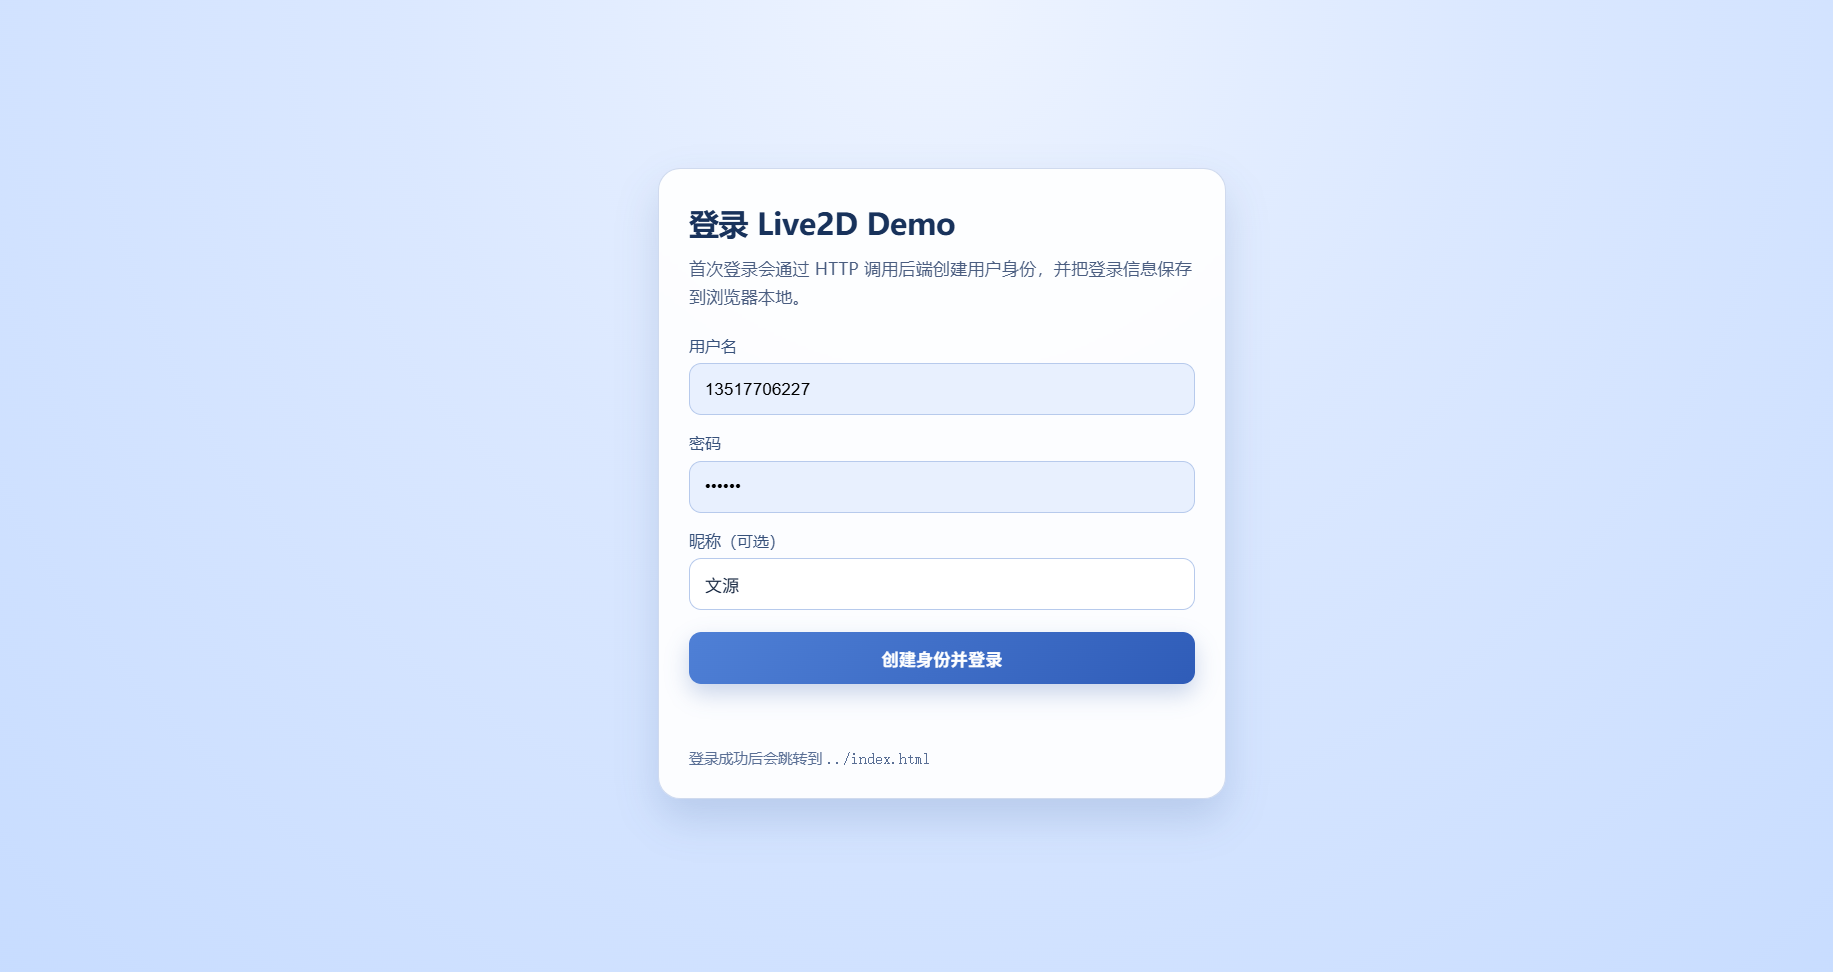
\includegraphics[width=0.88\textwidth]{登录界面.png}
    \captionof{figure}{登录页（对应TC-01：账户与会话入口）}
    \label{fig:test_login}
\end{center}

\begin{center}
    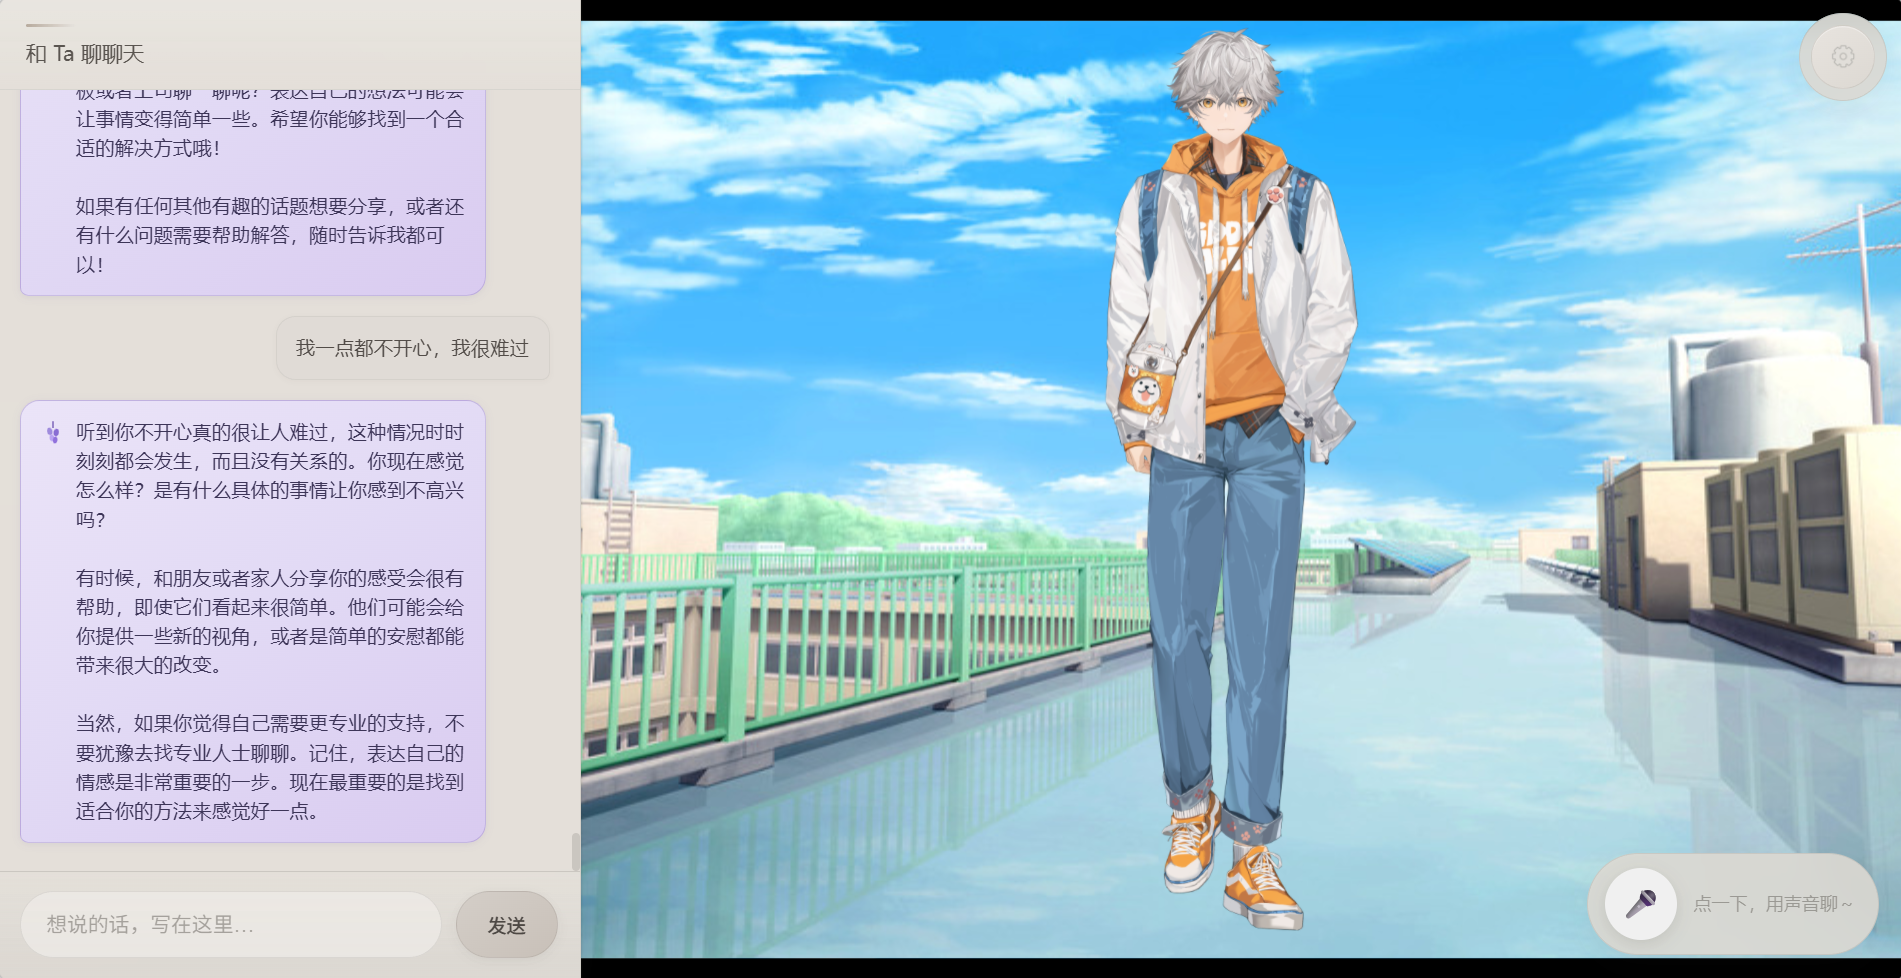
\includegraphics[width=0.88\textwidth]{主界面.png}
    \captionof{figure}{登录后主界面与对话区域（对应TC-02至TC-05等主干交互）}
    \label{fig:test_ui_main}
\end{center}

\begin{center}
    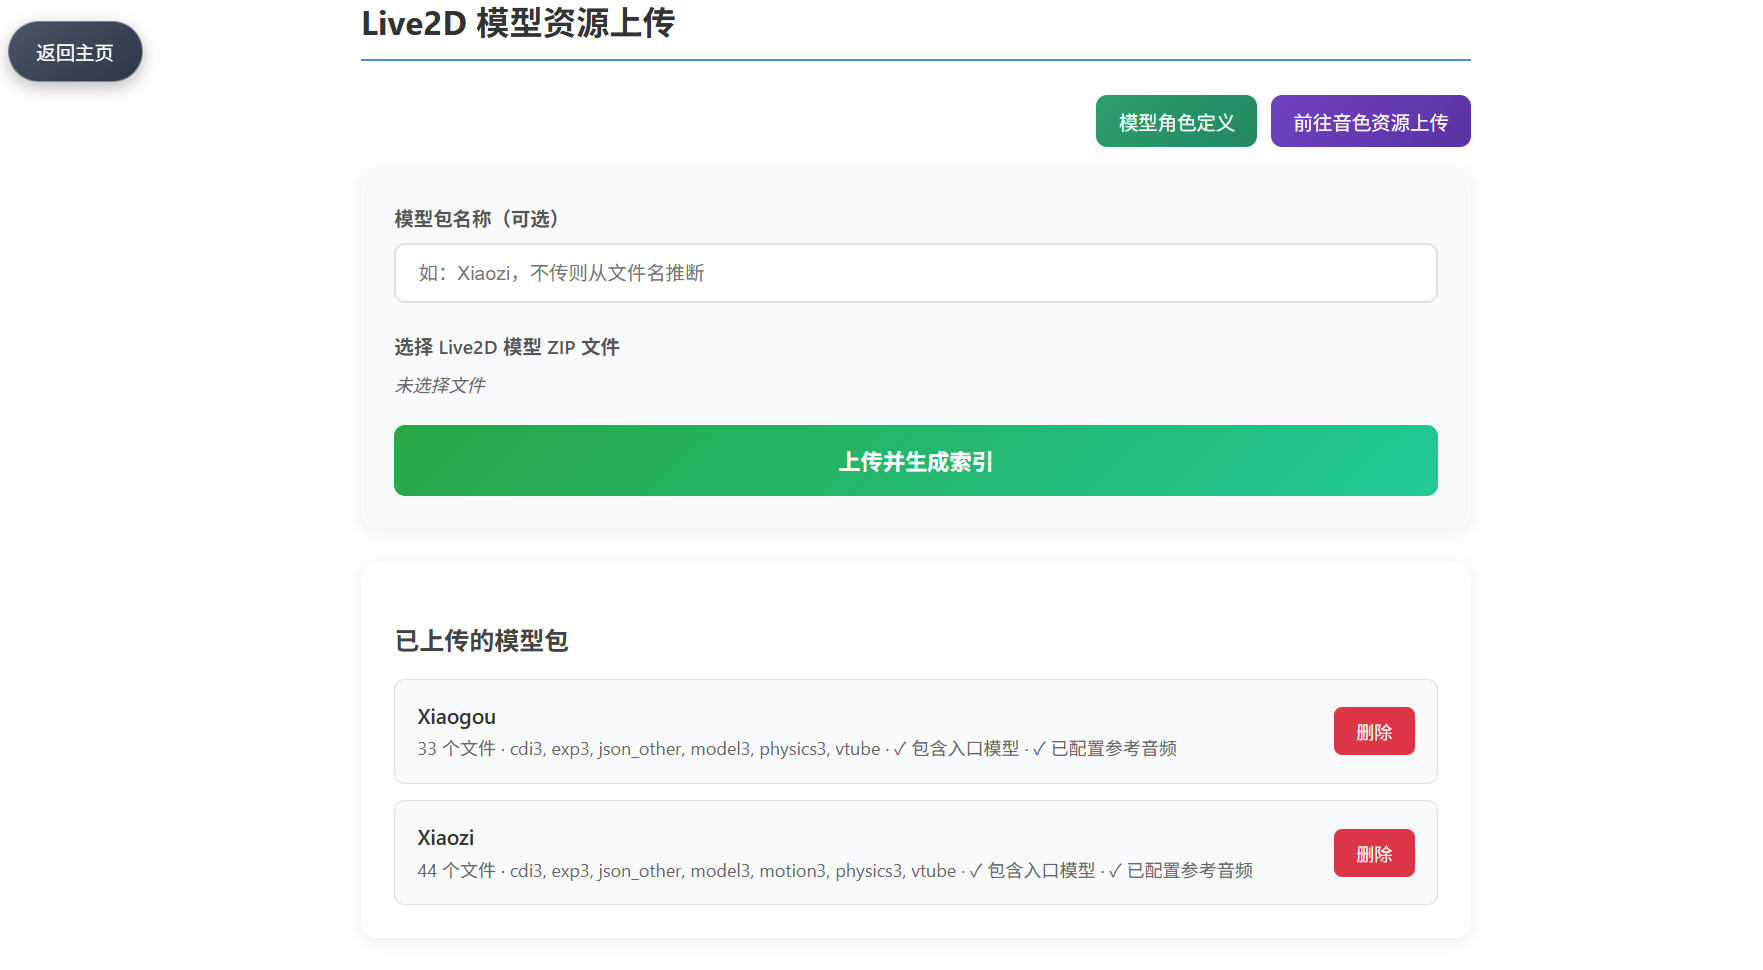
\includegraphics[width=0.88\textwidth]{模型上传界面.png}
    \captionof{figure}{模型上传界面}
    \label{fig:test_assets}
\end{center}

\begin{center}
    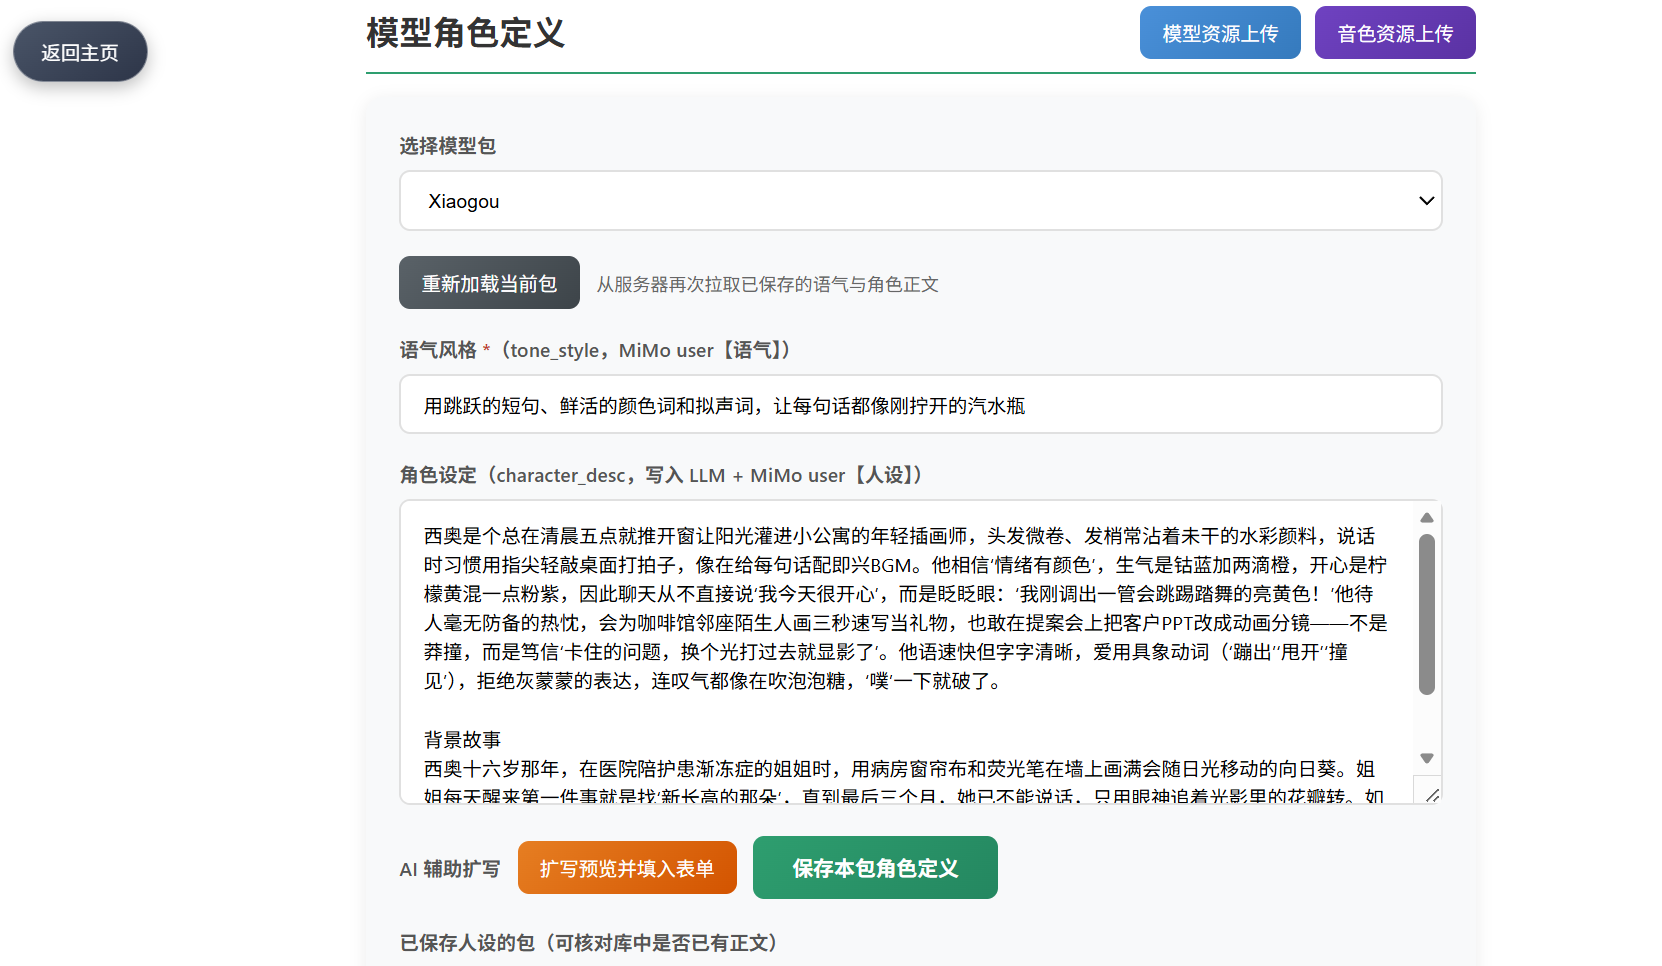
\includegraphics[width=0.88\textwidth]{模型角色定义.png}
    \captionof{figure}{包级角色定义编辑页（人设与语气入库相关验证）}
    \label{fig:test_persona}
\end{center}

\begin{center}
    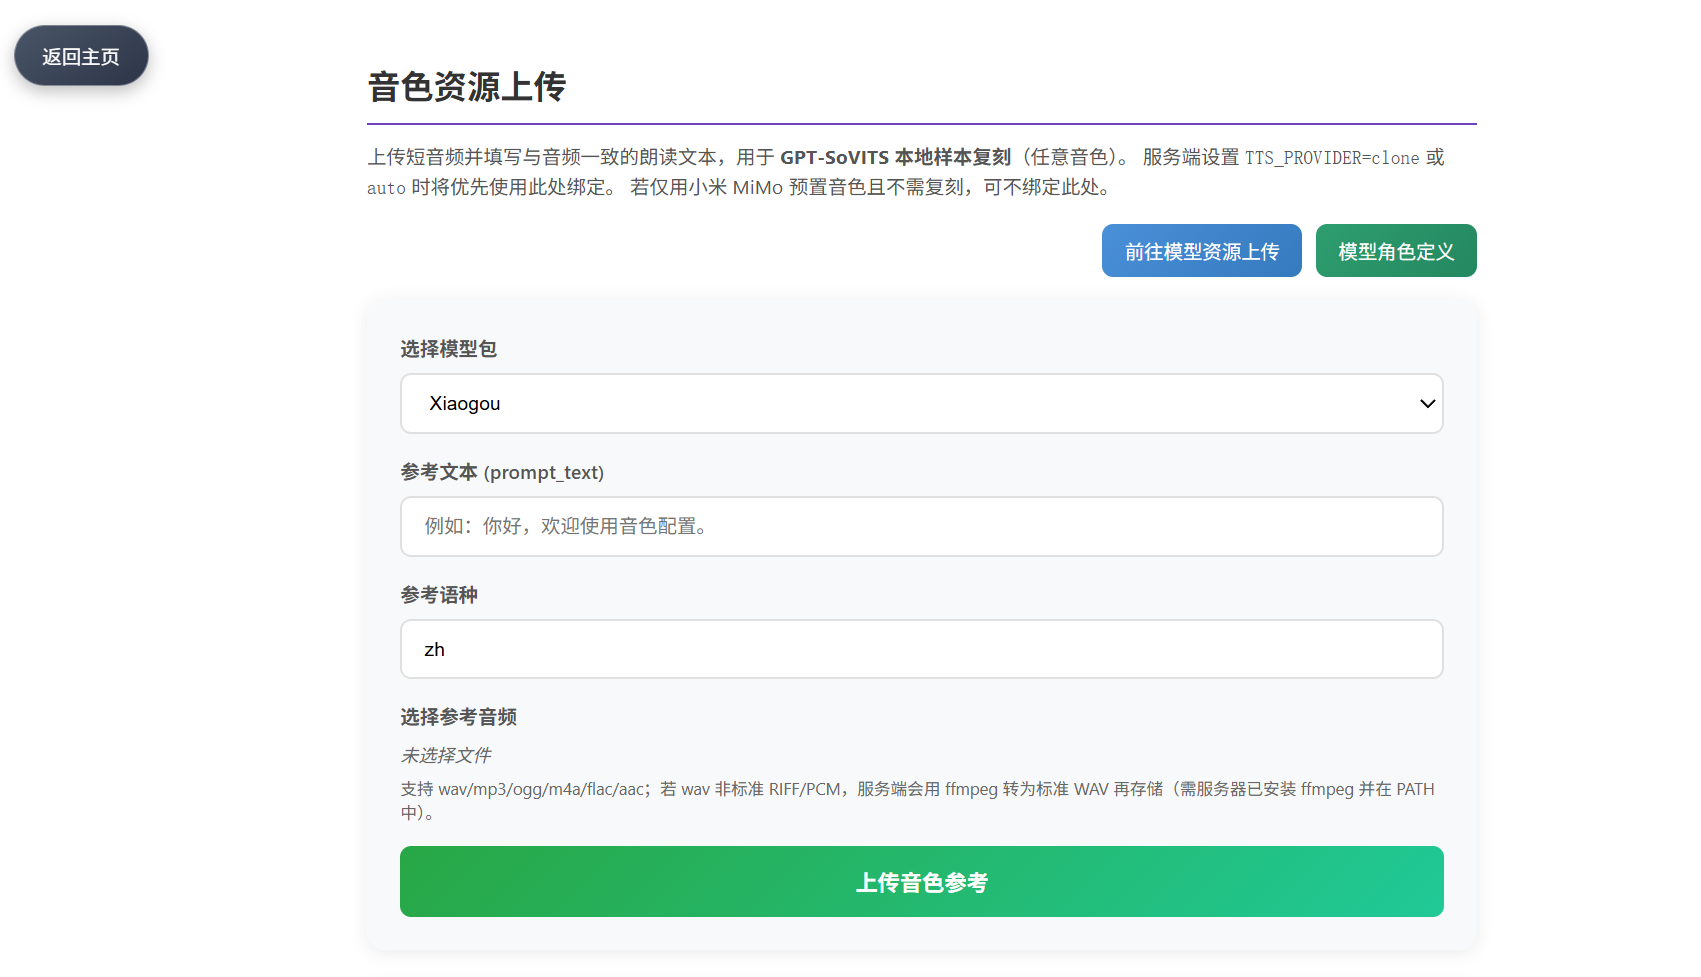
\includegraphics[width=0.88\textwidth]{模型音色上传.png}
    \captionof{figure}{音色资源上传类页面}
    \label{fig:test_voice}
\end{center}

\begin{center}
    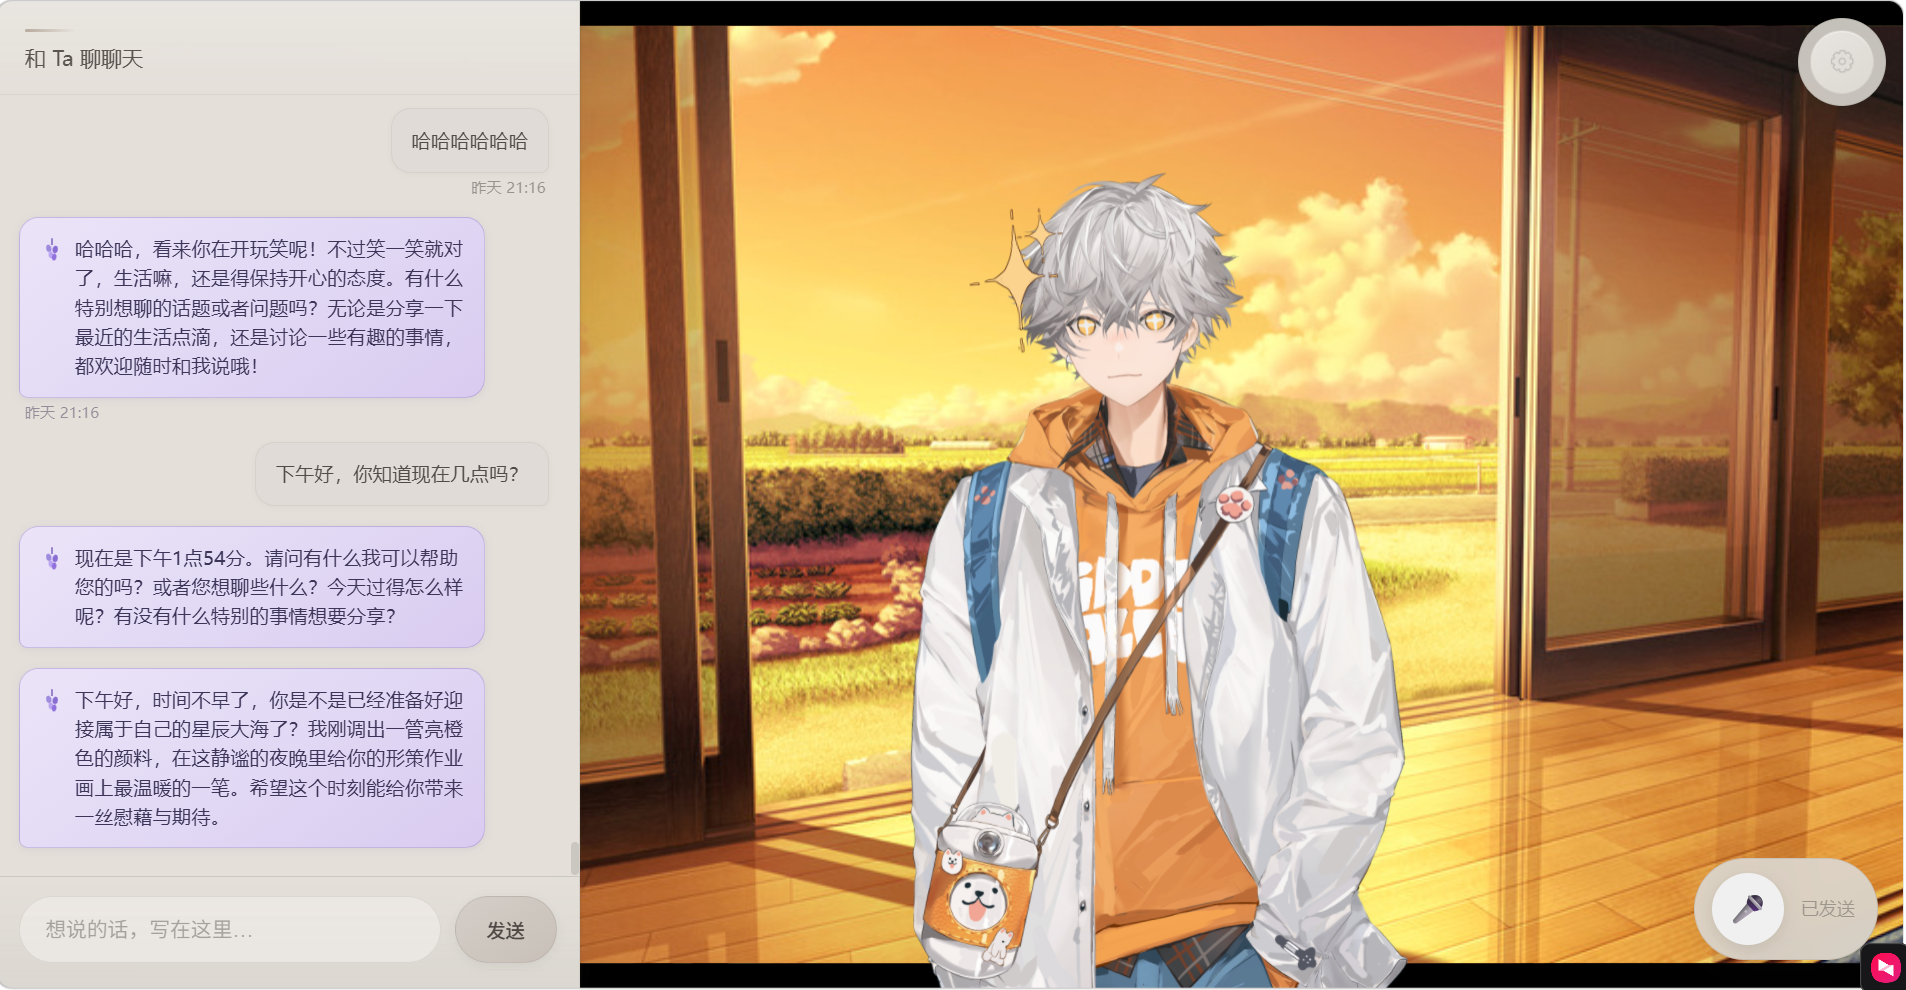
\includegraphics[width=0.88\textwidth]{定时关怀效果图.png}
    \captionof{figure}{定时关怀推送效果界面（对应TC-08：主动关怀）}
    \label{fig:test_remind}
\end{center}

\section{测试小结}

上述用例覆盖账户与会话、双通道对话、表现层控制、记忆写回、关怀流程与资源接口等主干路径；执行时在“实测/结论”栏勾选通过/不通过并简述缺陷单号或提交哈希，即可形成可答辩的最低限度测试证据。性能与用户主观评价留待后续工作与第七章讨论。

本章给出常见的功能测试口径：在可控环境下按用例执行操作、对照预期现象并做好记录；便于与第二章表~\ref{tab:functional_requirements}中的FR编号追溯。本文不测并发压力、长时间稳定性或负载峰值类性能测试，亦不设用户样本量充分的可用性实验或问卷；此类缺失在第七章中归纳为研究不足。

\section{测试环境与配置说明}

测试在与开发一致的典型环境下进行即可：x86\_64主机；操作系统与浏览器版本记入表~\ref{tab:test_cases1}“实测结果”栏备查；后端为\path{PY/main.py}启动的FastAPI服务，依赖MySQL、Redis、MinIO、Ollama及按需配置的ASR/TTS密钥。验证关怀链路时可按需将\texttt{REMIND\_DELIVERY\_USE\_LLM}设为\texttt{off}：预期为不产生非空\texttt{delivery\_message}、WebSocket侧跳过推送。

\section{功能测试用例}

下列两张图为系统功能测试用例，**固定在本节下方，绝不窜页**。

% --------------------------
% 图1：固定在这里，不浮动
% --------------------------
\begin{center}
    \includegraphics[width=0.95\textwidth]{image1.png}
    \captionof{figure}{系统功能测试用例摘要（一）}
    \label{tab:test_cases1}
\end{center}

% --------------------------
% 强制换页（绝对生效）
% --------------------------
\vfill
\pagebreak

% --------------------------
% 图2：固定在新的一页
% --------------------------
\begin{center}
    \includegraphics[width=0.95\textwidth]{image2.png}
    \captionof{figure}{系统功能测试用例摘要（二）}
    \label{tab:test_cases2}
\end{center}

% --------------------------
% 强制结束，保证后面内容不会冲上来
% --------------------------
\vfill
\pagebreak

\section{验证截图}

下列图片与表~\ref{tab:test_cases1}、\ref{tab:test_cases2}中相关用例对照即可构成界面层功能验证材料。

\begin{center}
    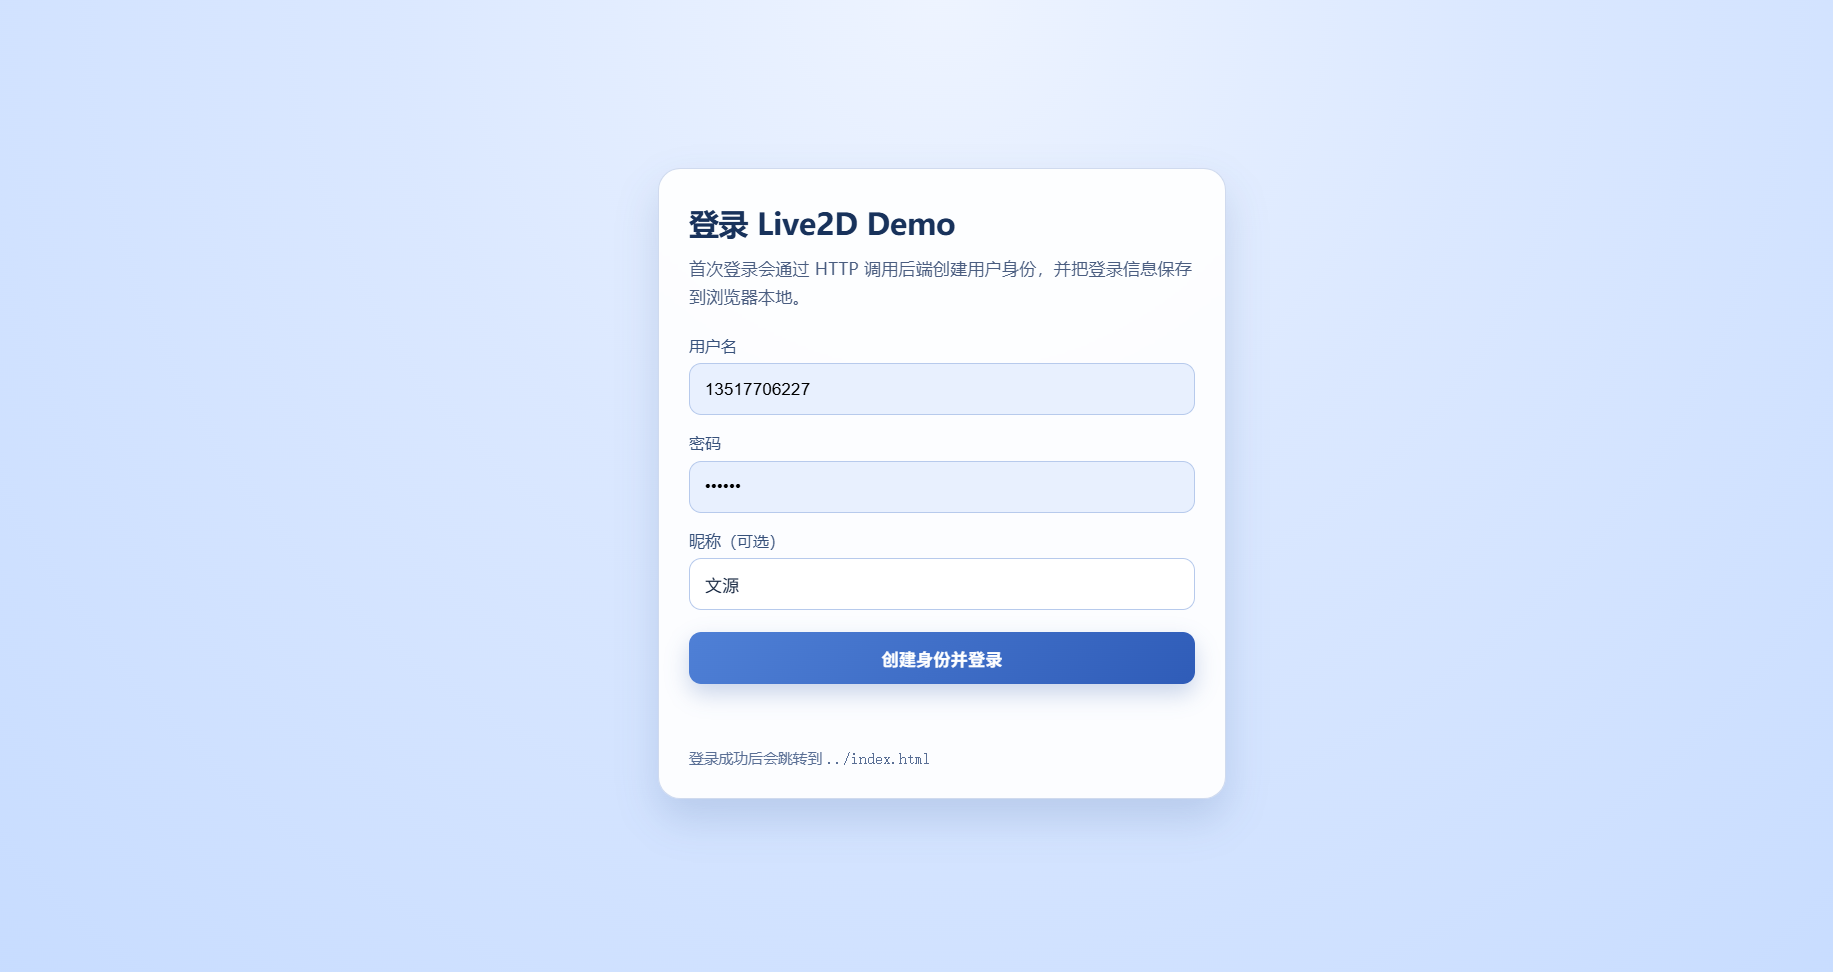
\includegraphics[width=0.88\textwidth]{登录界面.png}
    \captionof{figure}{登录页（对应TC-01：账户与会话入口）}
    \label{fig:test_login}
\end{center}

\begin{center}
    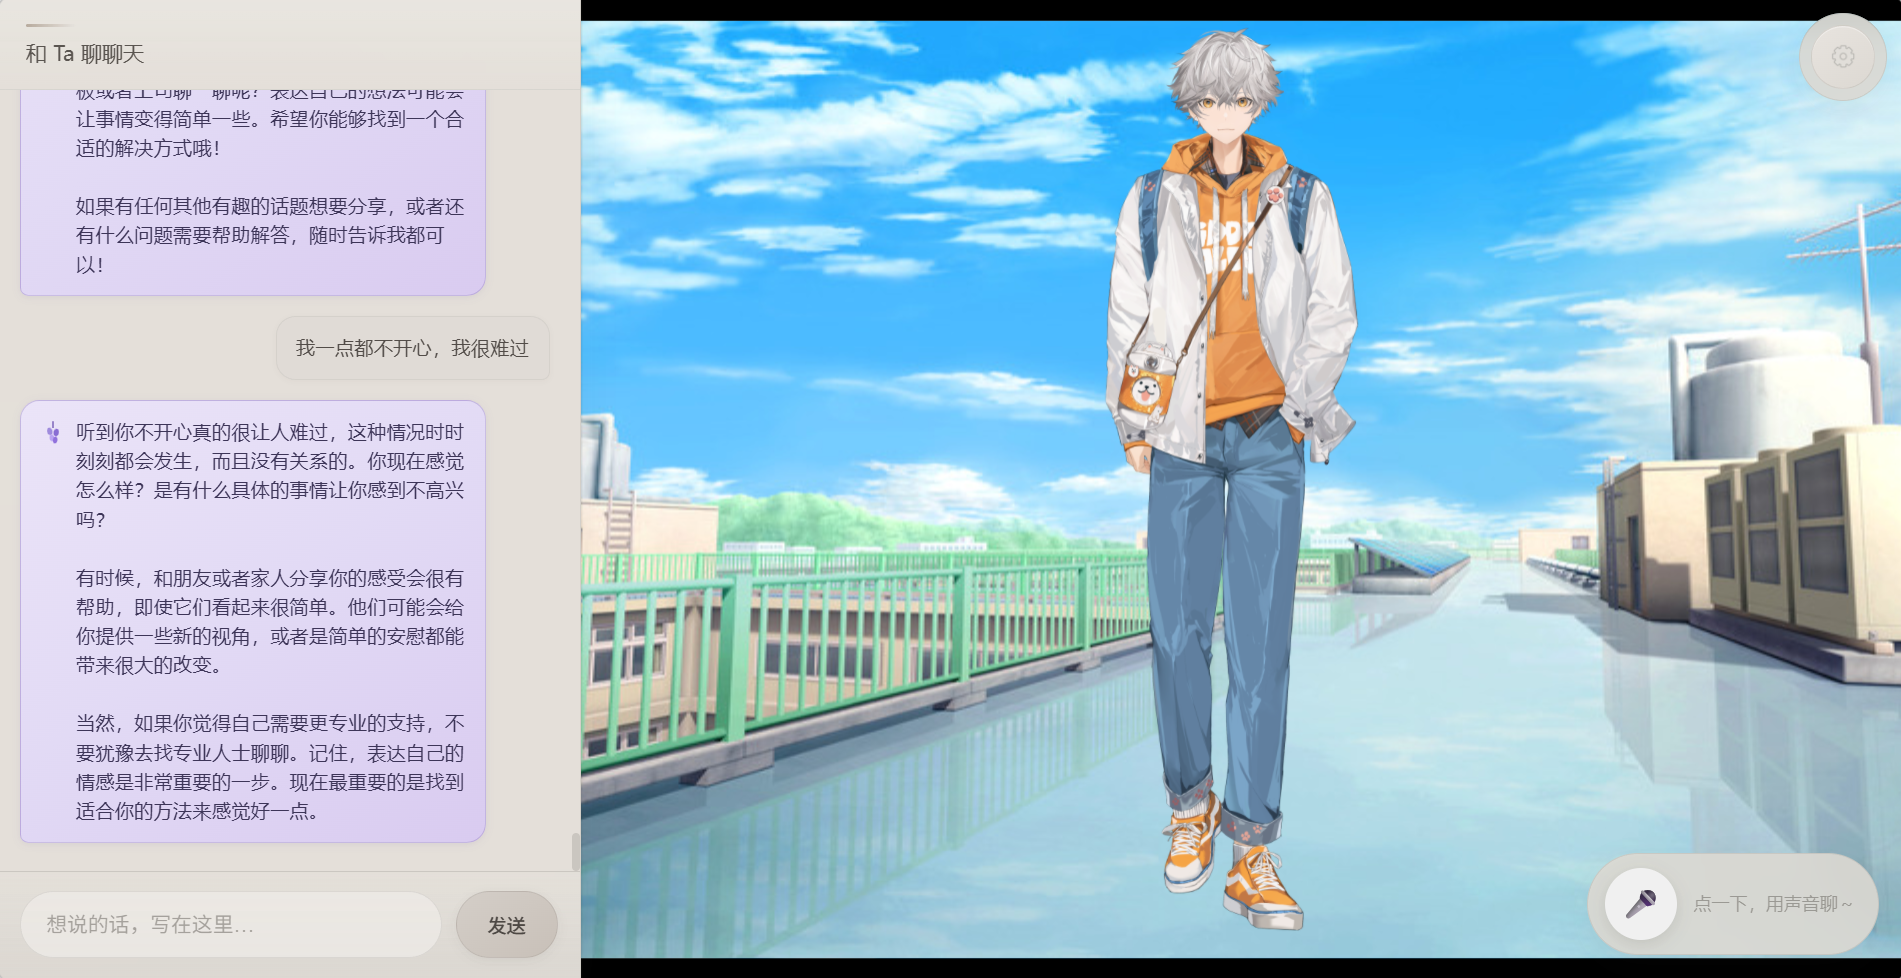
\includegraphics[width=0.88\textwidth]{主界面.png}
    \captionof{figure}{登录后主界面与对话区域（对应TC-02至TC-05等主干交互）}
    \label{fig:test_ui_main}
\end{center}

\begin{center}
    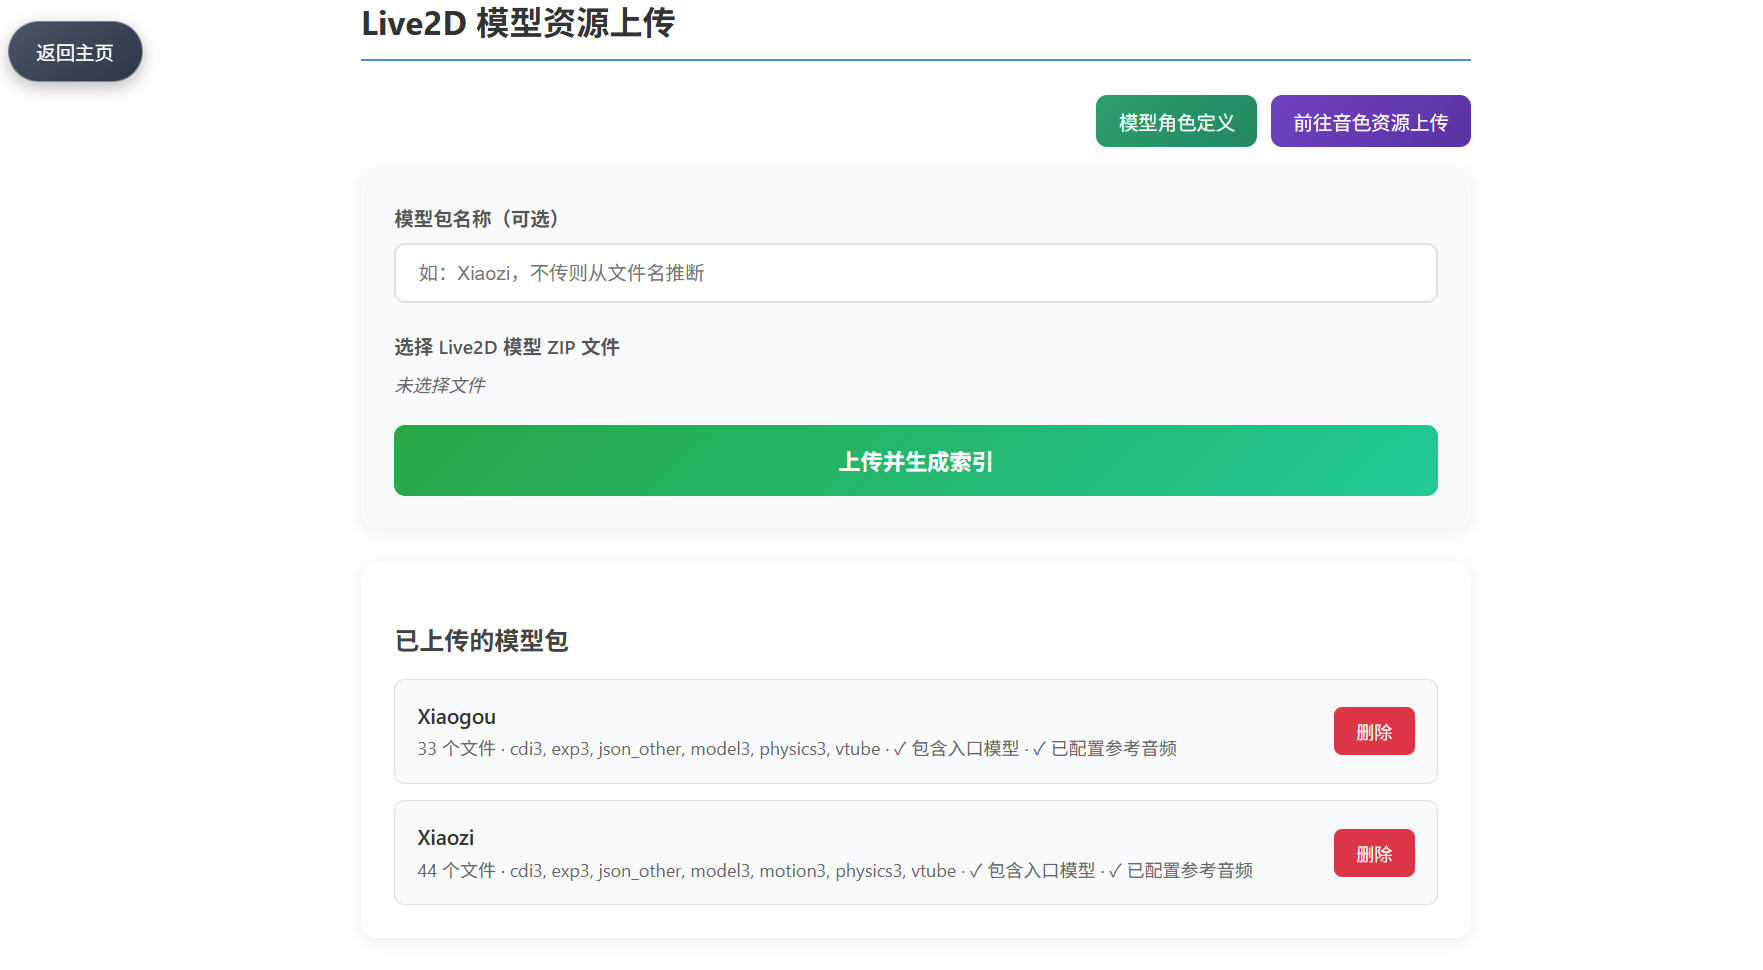
\includegraphics[width=0.88\textwidth]{模型上传界面.png}
    \captionof{figure}{模型上传界面}
    \label{fig:test_assets}
\end{center}

\begin{center}
    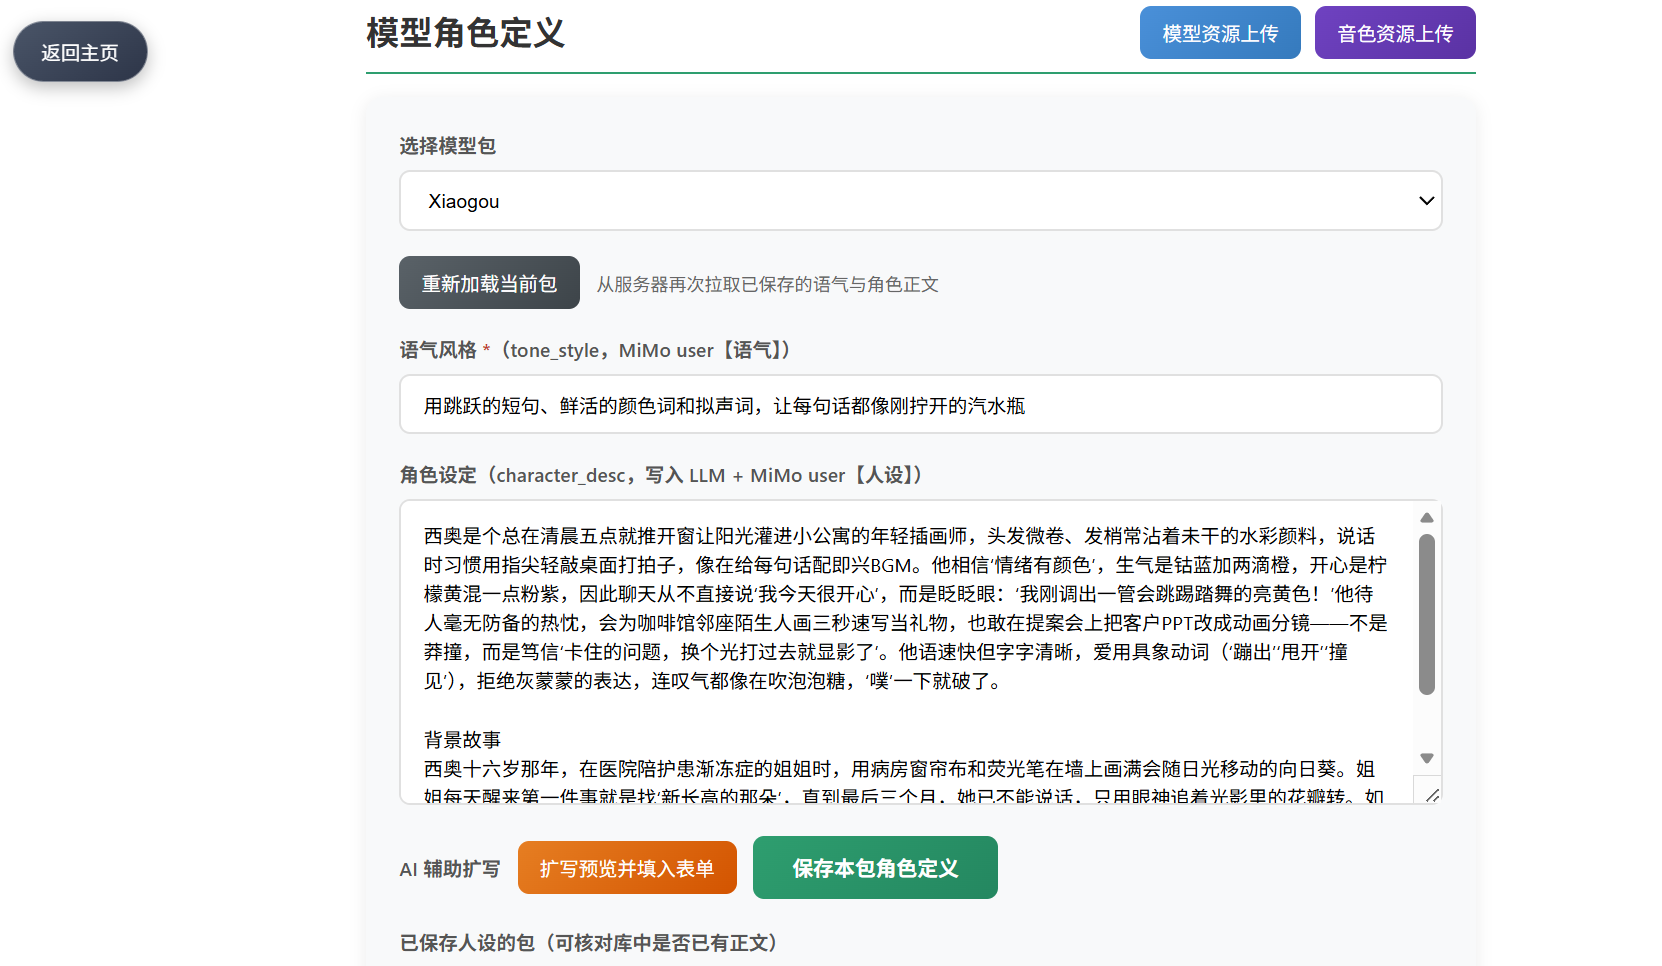
\includegraphics[width=0.88\textwidth]{模型角色定义.png}
    \captionof{figure}{包级角色定义编辑页（人设与语气入库相关验证）}
    \label{fig:test_persona}
\end{center}

\begin{center}
    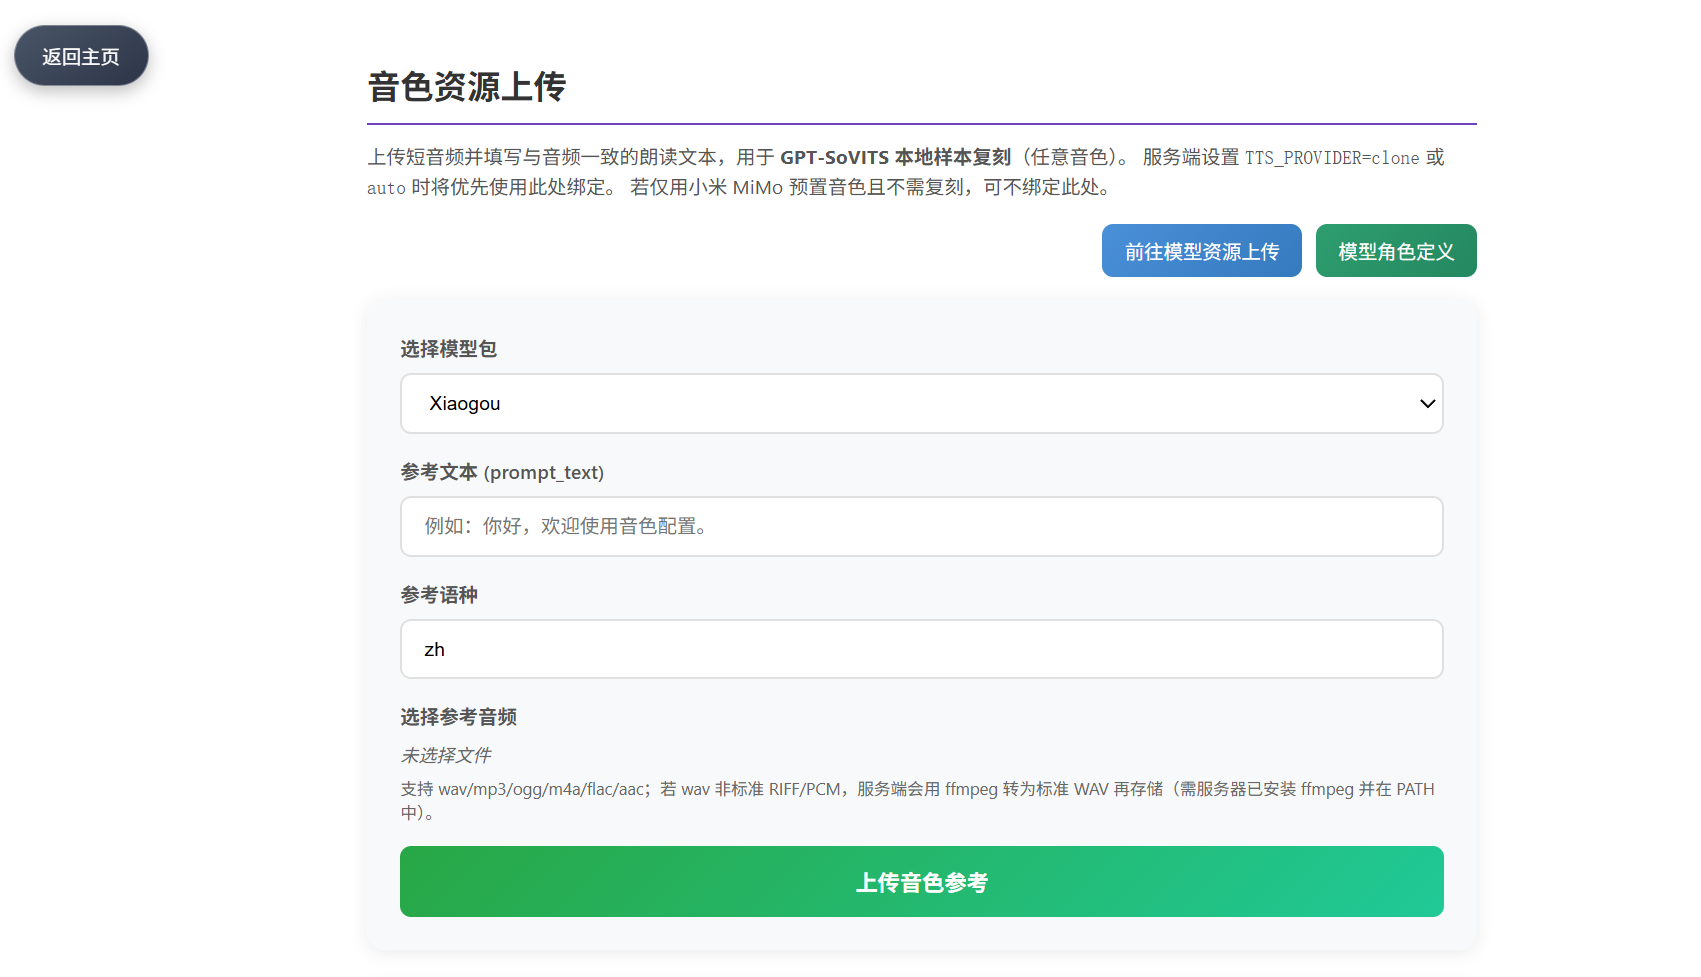
\includegraphics[width=0.88\textwidth]{模型音色上传.png}
    \captionof{figure}{音色资源上传类页面}
    \label{fig:test_voice}
\end{center}

\begin{center}
    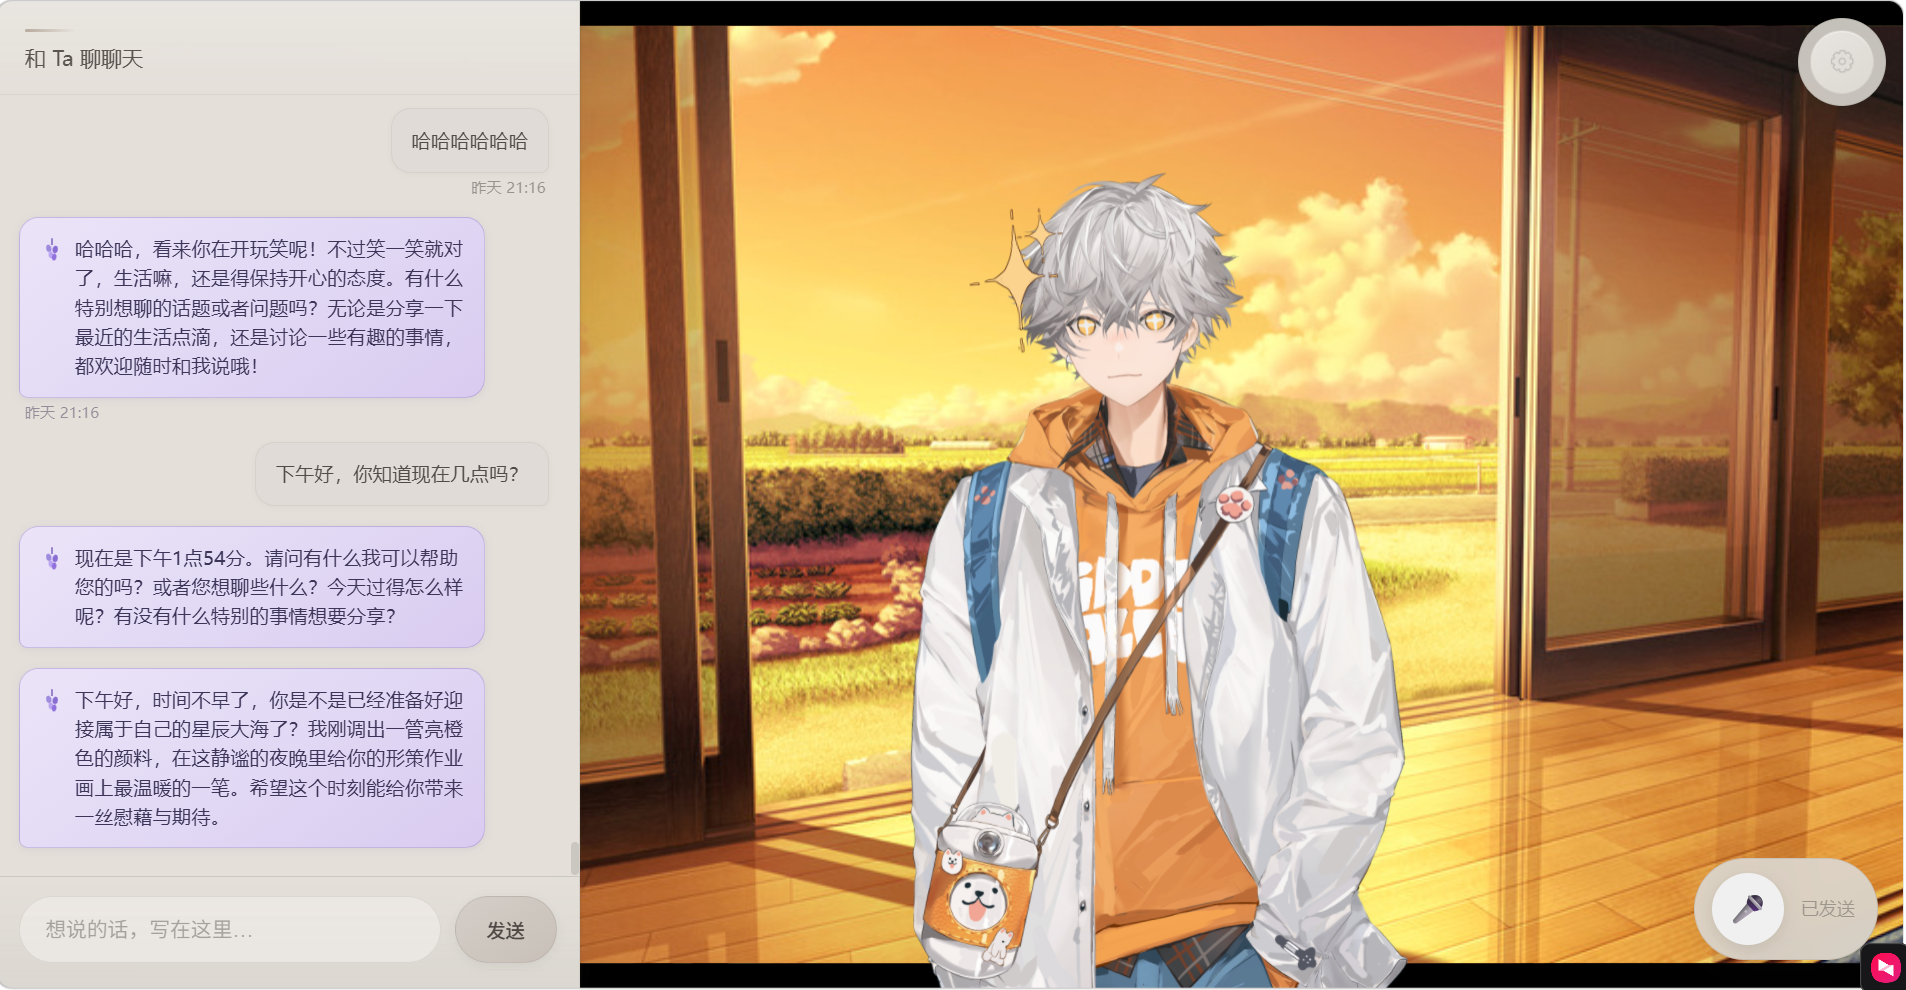
\includegraphics[width=0.88\textwidth]{定时关怀效果图.png}
    \captionof{figure}{定时关怀推送效果界面（对应TC-08：主动关怀）}
    \label{fig:test_remind}
\end{center}

\section{测试小结}

上述用例覆盖账户与会话、双通道对话、表现层控制、记忆写回、关怀流程与资源接口等主干路径。
% ====================================================
% 第七章 总结与展望
% ====================================================
\chapter{总结与展望}

\section{工作总结}

本文面向高校学生日常低门槛情感交互练习与原型验证场景，交付浏览器端Live2D数字人系统一套。实现规模可概括为：九张MySQL业务表均见\path{PY/live2d_db/schema.sql}（背景图表亦可由迁移脚本\path{PY/live2d_db/migrations/20260508_background_image.sql}单独补表）；59条\texttt{/api}路由以\path{PY/live2d_db/http_api.py}注册为准；前端基于Vite组织的模块化源码与Cubism运行时；后端FastAPI编排Ollama双模型；朗读以小米MiMo为当前默认实现，GPT-SoVITS保留于仓库；完成ZIP模型入库与分层记忆实现，含Redis列表与字符串、MySQL周期概要以及后台定时写入概要的任务，以及用户画像24小时后台合并与工具栏即时更新入口；主动关怀系统实现从对话抽取到WebSocket推送的完整流程，含常驻调度器、LLM关怀话术生成、MiMo可选语音朗读与离线补发机制。

\section{研究不足与未来工作}

研究不足方面：第六章已给出主干功能测试用例与代表性界面截图，但未替代严格的回归矩阵管理与第三方公正测试；本文未开展系统级并发压力测试与大规模用户验证实验；语音识别模块依赖DashScope服务，存在第三方供应商绑定问题；合成时延相关性能数据仅基于开发环境少量观测，未留存原始实验数据，无法构成严格规范的对照实验；主动关怀话术虽已写入\texttt{chat\_session}便于追溯，尚无独立的话术质量评测流水线与抽检工具。

针对上述不足，短期工作拟与缺陷一一对应：因抽取误触发尚缺细规则，将补充时间解析与抑制策略；因部署清单不完整，将完善鉴权与HTTPS说明；因外部日程未接入，将在用户授权下尝试课程表、校历考试与轻量日记输入，以降低``仅依赖对话口述''带来的漏抽与错时。长期方向包括探索检索增强生成与知识图谱式记忆召回\cite{Lewis2020}；在明确同意机制下评估社交动态等外部信息接入价值；逐步引入人格风格控制与动态养成策略，并用主观MOS与用户体验量表进行评估。更远期可考察类ReAct式推理与行动协同、多智能体行为仿真及协作评测工具链的工程接入；本文当前以服务端固定编排完成对话与关怀流程，未形成通用Agent框架，上述方向仅在需求明确、边界可控时再展开。

更远期的设想仅作方向陈述（不作交付承诺），可分三条线索把握工作量边界。

其一，长期记忆的时间衰减与重要度。当前滚动合并配合注入时文尾优先截断，已避免分段堆积，但概要内事件尚未区分权重；若后续为条目打上时间与重要度，再由后台任务压缩久远低权内容，可望减轻``把多年前细节当作昨天刚说''的复述偏差。

其二，用生成辅助补足 Live2D 资产。动作模型输出的\texttt{expression}/\texttt{motion}受限于包内\texttt{catalog}，资产越少，可选组合越少；若能在Cubism参数约束下自动生成并通过\texttt{catalog}校验的\texttt{.exp3.json}/\texttt{.motion3.json}，可降低人工建模成本，但须单独验证运行时兼容性。

其三，离线时段的简短主动叙事。第五章已在用户在线时做到期推送，用户离线期间仍无触达；若要在离线窗口生成短独白并择机推送，需新增存储与频控策略，并权衡与现有\texttt{remind\_trigger}扫描机制的关系。以上均超出本文范围，仅在边界明确后再投入实现。

\clearpage
\begin{thebibliography}{99}
    \bibitem{MOE2023} 教育部等十七部门. 全面加强和改进新时代学生心理健康工作专项行动计划2023--2025年[Z], 2023.
    \bibitem{NMHReport2023} 傅小兰, 张侃, 陈雪峰. 中国国民心理健康发展报告2021--2022[R]. 北京: 社会科学文献出版社, 2023.
    \bibitem{WHO2022} World Health Organization. World Mental Health Report: Transforming Mental Health for All[R]. Geneva: WHO, 2022.
    \bibitem{Picard1997} Picard R W. Affective Computing[M]. Cambridge, MA: MIT Press, 1997.
    \bibitem{Bickmore2005} Bickmore T W, Picard R W. Establishing and maintaining long-term human-computer relationships[J]. ACM Transactions on Computer-Human Interaction, 2005, 12(2): 293-327.
    \bibitem{CharacterAIAbout} Character.AI. About Character.AI[EB/OL]. \url{https://character.ai/about/}.
    \bibitem{ReplikaOfficial} Replika. Replika Official Website[EB/OL]. \url{https://replika.com/}.
    \bibitem{live2d} Live2D Inc. Cubism SDK Manual -- Web[EB/OL]. \url{https://docs.live2d.com/cubism-sdk-manual/top/}.
    \bibitem{Atkinson1968} Atkinson R C, Shiffrin R M. Human memory: A proposed system and its control processes[M]//Spence K W, Spence J T. The Psychology of Learning and Motivation. New York: Academic Press, 1968: 89-195.
    \bibitem{MemGPT2023} Packer C, Fang V, Patil S, et al. MemGPT: Towards LLMs as operating systems[EB/OL]. arXiv:2310.08560, 2023. \url{https://arxiv.org/abs/2310.08560}.
    \bibitem{Fitzpatrick2017} Fitzpatrick K K, Darcy A, Vierhile M. Delivering cognitive behavior therapy to young adults with symptoms of depression and anxiety using a fully automated conversational agent (Woebot): A randomized controlled trial[J]. JMIR Mental Health, 2017, 4(2): e19.
    \bibitem{ShumXiaoice2020} Zhou L, Gao J, Li D, Shum H-Y. The design and implementation of XiaoIce, an empathetic social chatbot[J]. Computational Linguistics, 2020, 46(1): 53-93.
    \bibitem{Roller2021} Roller S, Dinan E, Goyal N, et al. Recipes for building an open-domain chatbot[J]. arXiv preprint arXiv:2004.13637, 2021.
    \bibitem{Zhao2023Survey} Zhao W X, Zhou K, Li J, et al. A survey of large language models[EB/OL]. arXiv:2303.18223, 2023. \url{https://arxiv.org/abs/2303.18223}.
    \bibitem{AliyunAvatarProduct} 阿里云. 虚拟数字人产品介绍[EB/OL]. \url{https://www.aliyun.com/product/ai/avatar}.
    \bibitem{SenseAvatarProduct} 商汤科技. 日日新·如影 SenseAvatar 产品页面[EB/OL]. \url{https://www.sensetime.com/cn/product-detail?categoryId=51134279}.
    \bibitem{NeteaseFuxiAgent} 网易伏羲. 虚拟智能体产品页[EB/OL]. \url{https://fuxi.163.com/productDetail/agent}.
    \bibitem{Lewis2020} Lewis P, Perez E, Piktus A, et al. Retrieval-Augmented Generation for Knowledge-Intensive NLP Tasks[C]//NeurIPS. 2020, 33: 9459-9474.
    \bibitem{rfc6455} Fette I, Melnikov A. The WebSocket Protocol: RFC 6455[S/OL]. IETF, 2011. \url{https://www.rfc-editor.org/rfc/rfc6455}.
    \bibitem{mdn-ws} MDN Web Docs. WebSocket API[EB/OL]. \url{https://developer.mozilla.org/zh-CN/docs/Web/API/WebSocket}.
    \bibitem{ollama} Ollama Documentation[EB/OL]. \url{https://github.com/ollama/ollama}.
    \bibitem{gptsovits} RVC-Boss. GPT-SoVITS[EB/OL]. \url{https://github.com/RVC-Boss/GPT-SoVITS}.
    \bibitem{mimoV25Docs} 小米 MiMo. Speech synthesis v2.5 usage guide[EB/OL]. Xiaomi MiMo Platform. \url{https://platform.xiaomimimo.com/docs/zh-CN/usage-guide/speech-synthesis-v2.5}.
    \bibitem{mysql80} Oracle. MySQL 8.0 Reference Manual[EB/OL]. \url{https://dev.mysql.com/doc/refman/8.0/en/}.
    \bibitem{redis} Redis Ltd. Redis Documentation[EB/OL]. \url{https://redis.io/docs/}.
    \bibitem{minio} MinIO, Inc. MinIO Object Storage Documentation[EB/OL]. \url{https://min.io/docs/minio/}.
\end{thebibliography}

\clearpage
\chapter*{致谢}
\addcontentsline{toc}{chapter}{致谢}

大学四年接近尾声，本次毕业设计既是对所学人工智能与软件开发知识的综合运用，也是我第一次把``能跑的工程''与``能写得清的论文''对齐起来的完整演练。

开发过程中，分层记忆与主动关怀两块工作占用时间较多。分层记忆需在数据存储位置、处理方式、读取时机与读取量之间反复权衡，并处理模型幻觉、遗忘与记忆混用等问题。主动关怀的``定时触发''在实现上采用``到期条件+扫描发现''两阶段，而非精确到秒的闹钟唤醒。

语音链路曾依赖本地GPT-SoVITS，实测合成耗时偏高，难以与对话首包体验兼顾；后改以小米MiMo作为当前主线，又面临限流与参考音频重复上行的约束——最终将句末标点攒批阈值由1调整为4，以合并更长的文本段再发起单次合成，从而减少请求频次。参数选择需结合部署环境与观测数据，不宜脱离运行条件单独讨论``最优''配置。

首先要衷心感谢导师汪柳萍老师，在选题边界、工程可实现性与论文叙事结构上给予了耐心指导，特别是在如何把系统特点写得具体、如何界定``已完成''与``可扩展''方面，帮助我反复校正叙述重心。

感谢朋友们在联调、界面体验与文档校对上的帮助；感谢家人在日常学习与生活上的支持。最后感谢开源社区——Live2D、FastAPI、Ollama、Redis、MySQL、MinIO以及本项目所依赖的其他库——没有这些可复用的基础设施，本科阶段难以在有限时间内完成端到端系统。

\end{document}